\documentclass[a4paper, twoside]{report}

\usepackage[english]{babel}
\usepackage[utf8x]{inputenc}
\usepackage[T1]{fontenc}
\usepackage{listings}
\usepackage{hyperref}
\hypersetup{colorlinks=false}
\usepackage{lscape}
\usepackage{amsmath, amssymb}
\usepackage{graphicx}
\usepackage[dvipsnames]{xcolor}
\usepackage[colorinlistoftodos]{todonotes}

\usepackage{float}
\usepackage{colortbl}
\usepackage{subfigure}
\usepackage{amsthm}
\usepackage{mathtools}
\usepackage{tikz}
\usepackage{algorithm}
\usepackage{algpseudocode}
\usepackage{pseudocode}
\theoremstyle{definition}
\newtheorem{definition}{Definition}[section]
\newtheorem{thm}{Theorem}
%% Sets page size and margins
\usepackage[a4paper,top=3cm,bottom=2cm,left=3cm,right=3cm,marginparwidth=1.75cm]{geometry}

\makeatletter
\newcommand*{\centerfloat}{%
  \parindent \z@
  \leftskip \z@ \@plus 1fil \@minus \textwidth
  \rightskip\leftskip
  \parfillskip \z@skip}
\makeatother


\title{The Limits of Information Loss Metrics as Measures for Utility}
\author{Romain de Spoelberch}

\begin{document}
\begin{titlepage}

\newcommand{\HRule}{\rule{\linewidth}{0.5mm}} % Defines a new command for the horizontal lines, change thickness here

%----------------------------------------------------------------------------------------
%	LOGO SECTION
%----------------------------------------------------------------------------------------


\includegraphics[width=8cm]{title/logo.png}\\[1cm] % Include a department/university logo - this will require the graphicx package
 
%----------------------------------------------------------------------------------------

\center % Center everything on the page

%----------------------------------------------------------------------------------------
%	HEADING SECTIONS
%----------------------------------------------------------------------------------------
\quad\\[1.5cm]
%\textsc{\LARGE MSc Thesis}\\[1.5cm] % Name of your university/college
\textsc{\Large Imperial College London}\\[0.5cm] % Major heading such as course name
\textsc{\large Department of Computing}\\[0.5cm] % Minor heading such as course title

%----------------------------------------------------------------------------------------
%	TITLE SECTION
%----------------------------------------------------------------------------------------
\makeatletter
\HRule \\[0.4cm]
{ \huge \bfseries \@title}\\[0.4cm] % Title of your document
\HRule \\[1.5cm]
 
%----------------------------------------------------------------------------------------
%	AUTHOR SECTION
%----------------------------------------------------------------------------------------

\begin{minipage}{0.4\textwidth}
\begin{flushleft} \large
\emph{Author:}\\
\@author % Your name
\end{flushleft}
\end{minipage}
~
\begin{minipage}{0.4\textwidth}
\begin{flushright} \large
\emph{Supervisor:} \\
Yves-Alexandre de Montjoye 
% Uncomment the following lines if there's a co-supervisor
\\[1.2em] Florimond Houssiau
%\emph{Co-Supervisor:} \\
%Dr. Adam Smith % second marker's name
\end{flushright}
\end{minipage}\\[3cm]
\makeatother


%----------------------------------------------------------------------------------------
%	DATE SECTION
%----------------------------------------------------------------------------------------

% {\large A thesis submitted for the degree of}\\[0.5cm]
% {\large \emph{MSc Future Power Networks}}\\[0.5cm]
% {\large \today}\\[2cm] % Date, change the \today to a set date if you want to be precise

\vfill % Fill the rest of the page with whitespace

\end{titlepage}

\begin{abstract}
$k$-Anonymity is a popular privacy framework for the anonymization of tabular data, where one record is indistinguishable from at least $k-1$ others. This is typically done through generalization and suppression, with many degrees of freedom left to analysts. 

This allotted freedom gives rise to an exponential number of ways to $k$-anonymize a dataset. As a method to compare the utility of these different $k$-anonymous versions, a range of heuristic metrics have been proposed. However, the extent to which these metrics capture useful features of the data is unclear.

In this project, we propose the first assessment of these information loss metrics' power to predict utility in real-world tasks.

We consider simple machine learning tasks on several standard datasets, which we anonymize with state-of-the-art algorithms, varying a range of anonymization hyper-parameters.

We find that most metrics in the literature have tenuous links with utility, and that, between two $k$-anonymous versions of a dataset, trying to predict the one with more utility based on any individual metric only yields better-than-random results by 15\%, on average.

Following that, we train a model on the metrics to predict utility. This Meta-Metric represents the best case use for metrics, combining their predictive power. We show the Meta-Metric only improves our results by an additional 10\%. 
These results suggest that existing utility metrics are bad predictors for the utility of real-world tasks and cannot, in practice, guarantee the selection of the best anonymization procedure.
\end{abstract}

\renewcommand{\abstractname}{Acknowledgements}
\begin{abstract}
The lion's share of thanks go to Florimond Houssiau. He proposed the project, and generously devoted time every week to offer great advice. More than anything, his help taught me to think more creatively and analytically, a skill I hope to carry through no matter where I end up.

I would also like to thank Yves-Alexandre de Montjoye, whose ability to understand the crux of a problem, ask the right questions, and come up with creative solutions helped push this project forward and into new directions multiple times.

Of course, I also wish to thank my family for their unrelenting and unquestioning support, no matter what I get myself into. Finally, thanks to the Entity for making my days in Huxley ones that I'll never forget. 
\end{abstract}

\tableofcontents
% \listoffigures
% \listoftables

\chapter{Introduction}
In our increasingly digitalized world, every step of our day leaves a trace \cite{data_stats}. Per minute, Venmo-- a digital wallet that facilitates payments-- processes over $\$160,000$, each transaction containing information on both the sender and the recipient; Uber records over $9500$ rides, amassing information on users' movements, and AirBnB arranges $1500$ reservations. All this data can be used for good-- for example, in optimising services, or inferring how to better meet customers' needs.

Nevertheless, the collection of data poses privacy concerns. For example, recently, Google's project Nightingale has raised privacy red flags. The company, having struck a deal with one of America's largest healthcare provider, is getting the personal medical data of up to fifty million Americans \cite{guardian_data}. Their goals to further the field of medicine with data and artificial intelligence, laudable as they are, have left many suspicious. Some worry that the big tech company stands to gain a lot from using all of this information for alternative reasons, targeting individuals or selling the data, committing a major privacy breach in either case. 

Privacy concerns are taken seriously, as demonstrated by the 2016 European regulation: General Data Protection Regulation (GDPR). This regulation tightens control on data collection in Europe, and restricts the uses (processing) allowed \cite{gdpr_basic}. Along with a crackdown on what constitutes a privacy breach, GDPR includes Recital 26 \cite{recital26}, stating that the privacy measures instituted 
``should apply to any information concerning an identified or identifiable natural person''. Essentially, to use data like we used to, and to avoid the severe penalties put in place by the EU for privacy breaches, data must be anonymous. Where anonymity was important, ethically speaking, it is now mandatory.

Researchers have developed many anonymization methods to protect people's privacy, including one called $k$-anonymity \cite{kanon_orig}. $k$-Anonymization ensures that no individual in a dataset is distinguishable from $k-1$ others; it is often done by generalizing records -- removing detail from specific information so that individuals fit in the same broader categories. Additional privacy measures have to be put in place for the dataset to truly be considered anonymous but k-anonymization forms a good basis \cite{critique_kanon} and is widely used in the industry \cite{google2020anonymizing}.

There are exponentially many ways to $k$-anonymize a dataset, and each method entails the loss of varying amounts of information within the dataset. Analysts need datasets with as much preserved information as possible-- despite the coarsening of detail incurred-- to allow for accurate and diverse inferences. This is challenging and analysts cannot simply rely on their instincts. To solve this issue, researchers have presented a series of heuristic metrics that measure a proxy for the 
``utility'' of anonymized datasets \cite{ambiguity_metric, cm_granularity_metric, discern_metric, dse_metric, entropy_measure, hellinger&biv, ilm}.

These metrics have become pervasive in anonymization, and the attempt to maximize utility. For example, some $k$-anonymity algorithms are built with the aim of optimising for certain metrics like Sweeney's MinGen, optimising Precision \cite{kanon_algos}. Other algorithms, like Mondrian, are first presented with their results on existing information loss metrics to convince of their performance \cite{mondrian}. Anonymization toolboxes, like ARX, are available online. While they implement a hybrid version of multiple $k$-anonymization algorithms, they calculate a range of utility metrics for the anonymized dataset, leaving the metrics' importance up to the user \cite{arx}.

Although theses metrics are widely used, it is unclear whether they capture essential features of the data or if they can accurately judge a dataset's utility-- there is no evidence directly linking the metrics and utility. For that reason, in this project, we empirically test the correlation between the usefulness of a $k$-anonymous dataset, and its metric scores. We train off-the-shelf classifiers on the anonymous datasets, and equate these models' performances on real test data to utility. 

We create 600 anonymous versions of 4 datasets, heavily varied in terms of sizes and origins, using different hyperparameters (such as algorithm used, generalization trees, or the chosen $k$ value). 

We compare the models' performances to a wide range of utility metrics from the literature. Our results show that, taken individually, metrics are not good predictors for utility and any trend that can be observed is specific to the combination of dataset anonymized, algorithm used, and classifier used, implying very little applicability as general utility measures. We further tested whether the individual metrics could be used to choose the most useful of two $k$-anonymous versions of the same dataset. This is a situation that, currently, analysts will often rely on metrics for. The results show most metrics rarely outperform a random choice by more than 15\%. This suggests that the utility metrics commonly used to generate and evaluate anonymized datasets might not accurately predict the performances of simple machine learning tasks.


Finally, we propose an experiment to show that even in the best case, when an optimal combination of all our metrics is used, the metrics still do not have as much predictive power as implied in the literature:  we train a model to predict the accuracy of the classification task using the metrics, in a sense combining these metrics in a ``Meta''-Metric with as much predictive power as possible for a specific classification task. 

At their most predictive, the combination of metrics only improves our result by an additional 10\%. Additionally, we show these Meta-Metrics are task-specific; they are incapable of transferring their results to different datasets, different $k$-anonymization algorithms, or different classifiers. This means that ``expertise'' for a task is not transferable, and confirms that metrics are unusable as general utility measures.

\chapter{Background}
\section{k-Anonymity}
\subsection{Motivation}
When an organisation releases a dataset containing personal information, they are responsible for ensuring the privacy of all participants. This is not an easy task and, as research has shown time and time again \cite{sweeney_uniqueness, rocher_estimating_reid, kanon_orig}, a lot of public datasets fall short of this privacy expectation. For example, as a first step, many organisations release datasets in which any explicit identifiers like names are removed. Nevertheless, in a lot of cases, the remaining information can be used to re-identify individuals by using unique combinations of fields in the dataset. 

For instance, in a paper published in 2000, Latanya Sweeney showed that 87\% of partipicants in the 1990 U.S. Census survey were uniquely identifiable by a combination of their zipcode, gender, and age \cite{sweeney_uniqueness}. As such, if we had the U.S. Census dataset, and knew someone's age, address, and gender, chances are we could recover the rest of their personal data, in what Sweeney coined a re-identification by linking. In 2002, she published a paper demonstrating this attack \cite{kanon_orig}.

Linking two datasets, Sweeney managed to re-identify the medical records of William Weld, the governor of Massachusetts at the time. The first dataset was a health insurance dataset, including information such as ethnicity, procedures undergone, medications given, etc..., for all state employees in Massachusetts. Weld, as governor, was in the dataset. This information was pseudonymised, thought safe, and sold to industry. The second dataset was the Registered Voters list for Cambridge, Massachusetts: a publicly available record of registered state voters in Cambridge (Weld's county of residence). This contained names, addresses, party affiliations, etc... The two sets had three fields in common: zipcode, birthdate, sex.

Because the Voter List included names, Sweeney found Weld's details. According to her, six people in the health insurance set had Weld's birthday, and only three of them were men. When you took the zipcode into account, he was the only one left. As such, Sweeney could guarantee that the medical record was his.

Although these examples are old, they're not outdated. In 2019, Luc Rocher, et al., published a paper showing that over 99\% of Americans could be reidentified using 15 demographic attributes \cite{rocher_estimating_reid}. Although 15 pieces of information seems less dangerous than Sweeney's combination of age, sex, and zipcode, we now collect considerably more data than twenty years ago, making this just as threatening.


These experiments exemplify the danger of releasing pseudonymised datasets under the assumption they're safe. In the same paper that uncovers the Massachusetts governor's medical history, Sweeney proposes a measure to thwart linking attacks: k-Anonymity. Informally, in a k-anonymous dataset, no individual's record is distinguishable from at least $k-1$ others. This ensures that even having auxiliary information on an individual, an attacker will always find at least $k$ records with this information, creating uncertain links. 

 For example, table ~\ref{fig:basic_example} (a) displays 4 records in a dataset containing zipcodes, ages, and incomes. If we were to know someone's age and zipcode, we could unequivocally infer their income. Table (b) shows the result after a 2-anonymization. In this case, we achieved it by generalizing our records, making zipcodes less specific when necessary and giving age ranges instead of exact numbers. Even if we had auxiliary information on someone, we couldn't be certain about their income. For example, we want to find someone's salary, and we know their zipcode, and age: 79203, and 27 respectively. In (a), their income is 64k. In (b), we now can't differentiate row 2 and 4 since the ages have been generalized and the target's salary could equally be 98k or 64k. In this example, we arbitrarily used 2 as our k-value but any k bigger than one will confer some measure of security, increasing with k.

%Basic Example tables
\begin{figure}
\centering
\subfigure[$D$]{
    \begin{tabular}{|l|l|l|l|}
        \hline
        ID & Zipcode & Age & Income \\
        \hline
        1  & 28488      & 33  & 52k    \\
        2  & 79203      & 24  & 98k    \\
        3  & 28473      & 39  & 36k    \\
        4  & 79203      & 27  & 64k    \\
        \hline
    \end{tabular}}
\subfigure[$D'$, 2-Anonymous]{
    \begin{tabular}{|l|l|l|l|}
        \hline
        ID & Zipcode & Age & Income \\
        \hline
        1  & 284** & 30's  & 52k    \\
        \rowcolor{gray!50}
        2  & 79203      & 20's  & 98k    \\
        3  & 284** & 30's  & 36k    \\
        \rowcolor{gray!50}
        4  & 79203      & 20's  & 64k    \\
        \hline
    \end{tabular}}
\caption{An example of a small dataset, and a 2-Anonymous version of it. The indistinguishable records are shaded in the same hue.}
\label{fig:basic_example}
\end{figure}

\subsection{Notations and Definitions}
First, we establish the notation and definitions we'll use through the report. These will be consistent with those used in Sweeney's paper originally presenting k-Anonymity \cite{kanon_orig}.


We will only be dealing with structured data. We define a tabular dataset, $D$, as a collection of rows representing records. A record $x_i$ is an ordered tuple of attributes, $x \in (A_1 \times \dots \times A_m)$ and, thus, $D=\{x_i\}_{i=1}^{|D|}$. We write $D[S]$ to mean taking the subset $S$ of columns in $D$.

Whilst every attribute is unique --- that is, no two columns contain the same information --- a tuple can reappear multiple times throughout the data. Nevertheless, every tuple belongs to one person, and no person has two tuples in the dataset.

Attributes can be categorized into three subsets:
\begin{itemize}
    \item \textit{direct identifiers}: attributes that, by themselves, can fully identify an individual in a dataset. These include, but are not limited to: names, phone numbers, or email addresses.
    \item \textit{quasi-identifiers} (QI): Attributes that contain personal information but aren't sufficient alone to uniquely identify a person in the dataset. These are pieces of information like ages, genders, or zipcodes.
    \item \textit{sensitive attributes}: private information that should not be linked back to individuals. For example, salaries, or medical records.
\end{itemize}

For example, a dataset $D[name, zipcode, gender, age, illness]$ containing a Hospital's patient information has one direct identifer: $name$. The set of quasi-identifiers is $QI=\{zipcode, gender, age\}$, and finally, the sensitive attribute is $illness$.

\begin{definition}{k-Anonymity} \\
A table $D$, with quasi-identifiers $QI_D$, is k-anonymous if and only if each tuple in $D[QI_D]$ appears at least k times in $D[QI_D]$.
\end{definition}

We have formalized what we described in the motivation. We want any combination of quasi-identifiers to be indistinguishable from $k-1$ others. An equivalent definition is that any auxiliary information an attacker could gather would point to at least $k$ records, making re-identification harder.

\begin{definition}{Equivalence Classes} \\
An equivalence class in $D$ with respect to the quasi-identifiers, $QI_D$, is the set of records having identical values for $D[QI_D]$ \cite{mondrian}.
\end{definition}

In other words, the equivalence classes are the sets of records that have indistinguishable quasi-identifiers. In k-anonymous datasets, these classes have a cardinality of at least $k$. As an example, Table (a) in Figure ~\ref{fig:basic_example} has two equivalence classes: $\{1,3\}$ and $\{2,4\}$.

\subsection{Generalization and Suppression}
In this section, we formalize the theory of generalization, hinted at in the motivation.

At a first glance, k-anonymity could be achieved by removing all records that don't have equivalent classes of sufficient size. However, this can result in a lot of lost information. For that reason, most algorithms work with some form of generalization: instead of removing rows, tuples are replaced with more generic versions of them, allowing them to fit in broader equivalence classes \cite{kanon_algos}\cite{mondrian}. For example, in Figure ~\ref{fig:basic_example}, we achieve this by stripping the rightmost digits of a zipcode, thus referencing a larger geographical area, or by giving a range of ages instead of specific values. To formalize the way we approach attributes, and to facilitate the description of how to generalize them, we need to define a \textit{domain}:

\begin{definition}{Domain} \\
A domain is the set of values an attribute can take \cite{kanon_algos}. Domains can be continuous (e.g., a salary $\in \mathbb{R}$) or discrete (e.g., zipcodes $\subset \mathbb{Z}$ or categorical attributes like nationality: \{English, American, ...\}). The \textit{ground} domain of an attribute is the domain that hasn't been generalized at all. For instance, the ground domain of zipcodes, $Z_0$, is a string of any five digits. Domains can be generalized to make attributes less informative; say, $Z_1$ where $93772 \mapsto 9377*$. These build to become less and less specific $(Z_0, Z_1, Z_2...)$.
\end{definition}

We can see that for any domain, we need a function mapping every level of generalization to the next one -- i.e., for an attribute $A$, we need functions $\phi_i$ such that each is a generalization from a domain $A_i$ to the next generalized domain $A_{i+1}$. This will allow us to move from specific values to increasingly generalized ones. This is concept is formally respresented by \textit{Value Generalization Hierarchies}, and \textit{Domain Generalization Hierarchies}:

\begin{definition}{Value and Domain Generalization Hierarchy (VGH, DGH)}\\
For a quasi-identifier $A$, with a ground domain $A_0$, we need a set of surjective functions:

$$\phi_{A_i}: A_{i} \to A_{i+1}, \mbox{ for } i=0,...,n-1 \mbox{, such that } |A_n|=1$$ 

These functions reduce the size of the domain at every level, generalizing the values in them. This is called a Value Generalization Hierarchy ($VGH_A$).  

Additionally, we define the set of domains $\{A_i| i = 0,...,n\}$ as the Domain Generalization Hierarchy ($DGH_A$).
\end{definition}

The definition of a $VGH$ implies that every attribute is eventually generalized to a null value since $A_n$, the top level, only contains one element and everything must thus map to it. For example, going back to our zipcode example, if we assume every further generalization strips off the rightmost digit, we see that the highest level of generalization, $\phi_4$, maps any $x**** \mapsto *****$ and leaves us with a suppressed value; it divulges no information.

Intuitively, Value Generalization Hierarchies can be thought of as the generalization trees that will be used for values, Domain Generalization Hierarchies represent the actual values present at every level.

For example, Figure ~\ref{fig:tree_zip} displays the $DGH$ on $Z$, the zipcode attribute, if our dataset had a ground domain $Z_0 = \{x \in \mathbb{N} | 19300 \leq x < 19400 \}$. Notice that we go from $Z_2$ to total suppression. This is because $Z_2$ is singleton, implying further generalizations are pointless since we'll still have only one class of zipcodes.

%VHG Zip
\begin{figure}
\centering
\subfigure[$DGH_Z$]{
    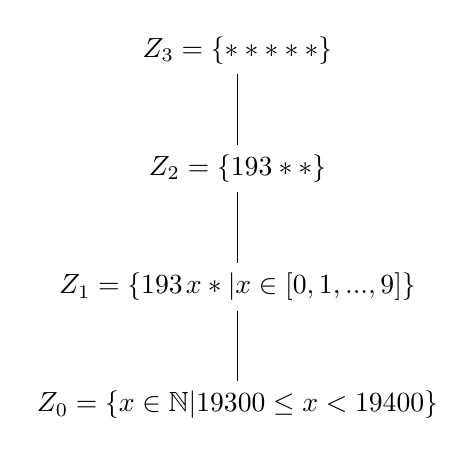
\begin{tikzpicture}[sibling distance=6em,
    level 2/.style={sibling distance=10em},
    level 3/.style={sibling distance=5em}]]
    \node {$Z_3 = \{*****\}$}
    child {node {$Z_2 = \{193**\}$}
    child {node {$Z_1 = \{193 \mspace{2mu}x* | x \in [0,1,...,9]    \}$}
    child {node {$Z_0 = \{x \in \mathbb{N} | 19300 \leq x < 19400 \}$}
    }}};
    \end{tikzpicture}}
\subfigure[$VGH_{Z}$]{
    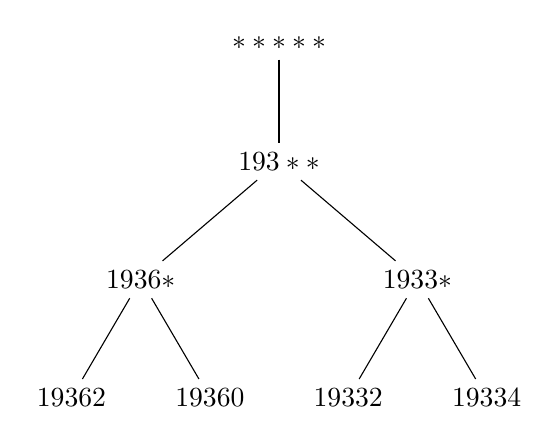
\begin{tikzpicture}[sibling distance=6em,
    level 2/.style={sibling distance=10em},
    level 3/.style={sibling distance=5em}]]
    \node {$*****$}
    child { node {$193**$} 
        child { node {$1936*$}
            child { node {$19362$}}
            child { node {$19360$}}
        }
        child { node {$1933*$}
            child { node {$19332$}}
            child { node {$19334$}}
        }
    };
    \end{tikzpicture}}
\caption{A DGH, and VGH for an example zipcode quasi-identifier}
\label{fig:tree_zip}
\end{figure}

It's important to point out that we can also create $VGH$s for categorical attributes. An example is provided in Figure ~\ref{fig:tree_ed}, with a level of education attribute $A_{ed}$ where we generalize the level of study to whether any further studies were undertaken after High School. The choice of the mapping is up to us, the data curators. For instance, we could also have decided that the difference between a Masters degree and a PhD was significant enough to warrant a third group, "Further Studies+" at the first level of generalization. This would give an alternative, but equally valid, VGH.

%VGH education
\begin{figure}
\centering
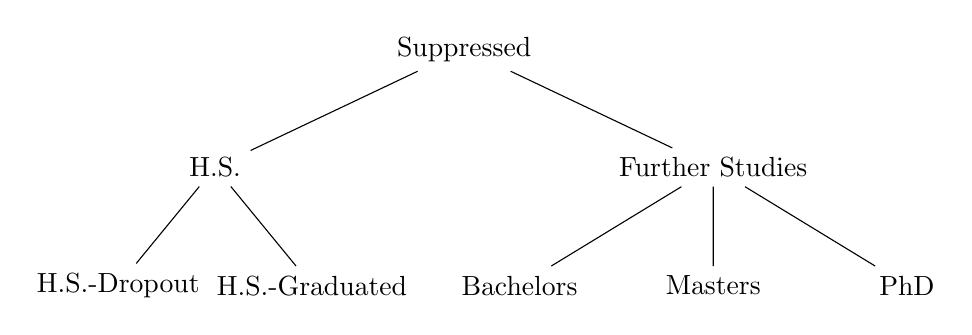
\begin{tikzpicture}[sibling distance=6em,
level 1/.style={sibling distance=18em},
level 2/.style={sibling distance=7em}]]
\node {Suppressed}
child { node {H.S.} 
    child { node {H.S.-Dropout}}
    child { node {H.S.-Graduated}}
}
child { node {Further Studies} 
    child { node {Bachelors}}
    child { node {Masters}}
    child { node {PhD}}
};
\end{tikzpicture}
\caption{An example VGH for a level of education attribute}
\label{fig:tree_ed}
\end{figure}

Finally, we introduce notation to define order in how generalized a dataset is:

\begin{definition}{Ordering Generalizations} \\ 
For a dataset $D$, and $D'$, a generalization of $D$. We introduce the notation $D \leq D'$ as a partial ordering meaning that $D'$ is a generalization of $D$. 
\end{definition}


\subsection{Existing Algorithms}

Because every $k$-anonymization involves generalizations and suppressions, although information does not change, it is coarsened, losing detail. We therefore aim to find algorithms that minimize how coarse the output is. However, we also have to take into account that there is a tradeoff with complexity -- if an algorithm takes too much time, then its applicability decreases. 

Before we can describe the algorithms, we introduce different generalization techniques that exist. The first is \textit{global single-dimensional generalization}:

\begin{definition}{Global Single-Dimensional Generalization} \\ 
On a table $D$ of size $n$, for an attribute $ A \in QI_D$, a global single-dimensional generalization on $A$ is the application of the functions defined for $VGH_A$ on the entire attribute column. We had defined a function at cell level so we extend the definition for an entire column with $n$ entries:  $\phi_{A_i}^{(n)}$, with $\phi_{A_i}^{(n)}: A_i^{(n)} \to A_{i+1}^{(n)}$, where $A_{i+1}$ is the next generalized domain. \cite{mondrian}

For example, reusing our defined VGH in Figure \ref{fig:tree_ed}, if our education column was as followed: $C_{ed_0} = ($Bachelors, PhD, PhD, H.S.-Graduated$)$, then a Global Single-Dimensional Generalization returns $C_{ed_1}$:
\[C_{ed_1} = (\text{Further Studies, Further Studies, Further Studies, H.S.})\]
We can generalize $C_{ed_1}$ one step further, to suppression:
\[C_{ed_2} = (\text{Suppressed, Suppressed,Suppressed,Suppressed})\]

This type of generalization is single-dimensional, meaning it has a specific mapping for every quasi-identifier defined in the VGH, and global because it generalizes an entire attribute column at once.
\end{definition}

To allow for more flexibility, we can generalize on combinations of a table's quasi-identifiers:
\begin{definition}{Global Multidimensional Generalization} \\ 
Let $D$ be a dataset with quasi-identifiers $(A_1,...,A_n)$. Instead of having a function per quasi-identifier, we define a single function $\phi: A_1 \times ... \times A_n \to A_1' \times ... \times A_n'$ that generalizes by the record. The only requirement is that $A_i'$ is equally as general or moreso than $A_i$. This allows for more flexible generalizations as we don't need to ensure every column is $k$-anonymous independently.

For example, take Figure \ref{fig:multi_vs_singledim_example}. $D''$ is a $2$-anonymous version of $D$ done using a global multidimensional generalization. We see that its Zipcode column isn't generalized to the same extent for every value, leaving us with more detail than in $D'$, anonymized by applying single-dimensional generalizations.
\end{definition}

%multi vs. single dimensional Example tables
\begin{figure}
\centering
\subfigure[$D$, A dataset]{
    \begin{tabular}{|l|l|l|}
        \hline
        Zipcode & Age & Income \\
        \hline
        28498 & 30's  & 52k    \\
        79203 & 20's  & 98k    \\
        28473 & 30's  & 36k    \\
        79203 & 20's  & 64k    \\
        \hline
    \end{tabular}}
\subfigure[$D'$, Global Single-Dimensional Generalization]{
    \begin{tabular}{|l|l|l|}
        \hline
        Zipcode & Age & Income \\
        \hline
        284** & 30's  & 52k    \\
        284** & 30's  & 36k    \\
        \rowcolor{gray!50}
        792**      & 20's  & 98k    \\
        \rowcolor{gray!50}
        792**      & 20's  & 64k    \\
        \hline
    \end{tabular}}
\subfigure[$D''$, Global Multidimensional Generalization]{
    \begin{tabular}{|l|l|l|}
        \hline
        Zipcode & Age & Income \\
        \hline
        284** & 30's  & 52k    \\
        284** & 30's  & 36k    \\
        \rowcolor{gray!50}
        79203      & 20's  & 98k    \\
        \rowcolor{gray!50}
        79203      & 20's  & 64k    \\
        \hline
    \end{tabular}}
\caption{An example demonstrating the difference between a single-dimensional and a multidimensional global generalization on table $D$. Equivalence classes are shaded in the same hue. We notice that we can preserve more detail on the zipcode attribute by generalizing Multidimensionally.}
\label{fig:multi_vs_singledim_example}
\end{figure}

The alternative approach is to attempt generalization locally. For example, we can partition our dataset into a \textit{multi-dimensional region}:

\begin{definition}{multi-dimensional region} \\
On a table $D$, with quasi-identifiers $A_1, A_2, ..., A_m$. Assuming a total order on these attributes, we can partition the dataset into regions defined by a pair of tuples $(l_1, ..., l_m),(u_1,...,u_m) \in A_1\times A_2\times ... \times A_m$ such that $\forall i, l_i \leq u_i$ \cite{mondrian}. Intuitively, this equates to partitioning $D$ into $m$-dimensional rectangular boxes that cover the state-space. 

The generalizing function $\phi$ maps each tuple $(x_1, ..., x_m) \in A_1\times A_2\times ... \times A_m$ to a summary statistic of the region it contains. These summary statistics can take many shapes, the simplest one being a range of values present in the region. 
\end{definition}

From the many algorithms that have been proposed, (\cite{ola_algo}\cite{mondrian}\cite{incognito}\cite{kanon_algos}), we'll describe a few of particular interest: MinGen, Datafly, and Mondrian. Datafly is the first algorithm proposed by Sweeney \cite{sweeney_datafly}. She later introduced MinGen, the first algorithm optimised for a utility metric,  and, finally, Mondrian-- an efficient local generalization algorithm \cite{mondrian}. 

\subsubsection{DataFly: Greedy Single-Dimensional Generalization}
In 1997, before formalizing the concept of k-anonymization, Sweeney developed a practical anonymization algorithm called Datafly \cite{sweeney_datafly}. Datafly works by greedily generalizing the quasi-identifier with the largest domain, using a Global Single-Dimensional approach. It does so iteratively, until the table is k-anonymous, or close enough to warrant suppressing a few records. 

For a dataset $D$, the algorithm revolves around a frequency table of the tuples in $D[QI_D]$. Whilst more than k records in the frequency table are not anonymous, Datafly will generalize an attribute, and update the frequency table accordingly. At the end, the small amount of leftover non-anonymous records are removed, and the dataset is rebuilt from the frequency table -- i.e., a tuple with a certain count is inserted that many times in a new table. The following is outlined in Algorithm \ref{datafly}. In this pseudo-algorithm, \textit{generalize} means to globally and single-dimensionally generalize the attribute with the generalization function from the VGH with the appropriate depth.
%Datafly
\begin{algorithm}
\caption{Datafly: a practical k-anonymization}
\label{datafly}
\textbf{Input:} Table $D$; a defined $DGH$ for every $QI$; a fixed k. \\
\textbf{Output:} $D'$, a k-anonymous generalization of $D$
\begin{algorithmic} % enter the algorithmic environment
    \Ensure $|T| > k$
    
    \State freq $\leftarrow \{\forall t \in T[QI_T]: (t, count(t, T[QI_T]))\}$     
    \While{more than k tuples in freq are not k-anonymous}
        \State $A_j \leftarrow \max_{A \in QI}(|\{\mbox{freq}[A]\}|)$ 
        \State freq$[A_j] \leftarrow generalize($freq$[A_j])$
    \EndWhile
    \State freq $\leftarrow$ suppress tuples occuring less than k times
    \State $GT \leftarrow rebuild($freq$)$ \\
    \Return $GT$
    
\end{algorithmic}
\end{algorithm}

This algorithm is fast but may distort data more than necessary due to the fact it makes ``crude decision'' in generalizing entire columns at once. Furthermore, it heavily penalizes attributes with a wide range of different values, leading to unecessary generalizations. For example, if we had a table $D(ZIP, gender)$, our domain $ZIP_4$, containing things of the form x**** would contain up to 10 different elements whereas $gender_0$ would have two at most. This means that before Datafly even considers generalizing gender, it would fully suppress the zipcode.


\subsubsection{MinGen: Minimal Generalization}
\label{mingen}
As mentioned above, we are looking to keep our data as integral as possible and Datafly doesn't always satisfy that requirement. To rectify that, Sweeney proposed MinGen in 2002\cite{kanon_algos}. MinGen is naive, and "makes no claim to be efficient" but guarantees k-anonymity with the minimal amount of generalization over the quasi-identifiers using global single-dimensional generalizations. 

We define minimal generalization:

\begin{definition}{k-Minimal Generalization} \\
Let $D_l(A_1,...,A_n)$ and $D_m(A_1,...,A_n)$ be two tables such that $D_l[QI] \leq D_m[QI]$ where $QI$ is the set of quasi-identifiers associated with the tables. $D_m$ is said to be a k-minimal generalization of $D$ over $QI$ if and only if:
\begin{itemize}
    \item $D_m$ satisfies the k-anonymity property
    \item $\forall$ k-anonymous $D_z$ satisfying $D_l \leq D_z$ and $D_z \leq D_m$ then $D_z = D_m$. 
\end{itemize}
\end{definition}

In other words, this definition helps us find the first generalized table that is k-anonymous. Nevertheless, every table could have multiple k-minimally generalized tables, and they wouldn't all be as useful. For example, Table \ref{fig:kminimal_gen_tables} depicts two different k-minimal generalizations of a Table $D$: we could either generalize zipcode by removing the last three digits, or by generaling both zipcode and age once. They're both 2-anonymous, and any $G$ with $G \leq D'$ or $G \leq D''$ wouldn't be, implying 2-minimal generalization. The question now becomes, which should we use?

%Min generalization example
\begin{figure}
    \centering
    \subfigure[$D$]{
    \begin{tabular}{|c|c|}
    \hline
    Zipcode & Age \\
    \hline
    97385 & 21 \\
    97412 & 21 \\
    97492 & 36 \\
    97365 & 36 \\
    \hline
    \end{tabular}}
    \subfigure[$D'$]{
    \begin{tabular}{|c|c|}
    \hline
    Zipcode & Age \\
    \hline
    973** & [20-40] \\
    974** & [20-40] \\
    974** & [20-40] \\
    973** & [20-40] \\
    \hline
    \end{tabular}}
    \subfigure[$D''$]{
    \begin{tabular}{|c|c|}
    \hline
    Zipcode & Age \\
    \hline
    97*** & 21 \\
    97*** & 21 \\
    97*** & 36 \\
    97*** & 36 \\
    \hline
    \end{tabular}}
    \caption{Different $k$-minimal generalizations for a table $D$. $D'$ generalizes twice on zipcode and once on age. Revert any of these generalizations and our table is no longer $2$-anonymous, implying it is a minimal generalization. Instead, $D''$ generalizes further on the zipcode but leaves age untouched. It is also a $2$-minimal generalization.}
    \label{fig:kminimal_gen_tables}
\end{figure}

To solve that, Sweeney, et al., define a preference criteria in the form of the precision metric (defined in \nameref{metrics_prec}) which captures the amount of information lost and we define minimal distortion:

\begin{definition}{k-Minimal Distortion} \\
Let $D_l(A_1,...,A_n)$ and $D_m(A_1,...,A_n)$ be two tables such that $D_l[QI] \leq D_m[QI]$ where $QI$ is the set of quasi-identifiers associated with the tables. $D_m$ is said to be a k-minimal distortion of $D$ over $QI$ if and only if:
\begin{itemize}
    \item $D_m$ satisfies the k-anonymity property
    \item $\forall$ k-anonymous $D_z$ satisfying $Prec(D_l) \geq Prec(D_z)$ and $Prec(D_z) \geq Prec(D_m)$ then $D_z = D_m$. 
\end{itemize}
\end{definition}

Furthermore, Sweeney states as a Theorem: 
\begin{thm}\cite{kanon_algos}
    Given datasets $D_l$ and $D_m$ such that $D_l \leq D_m$, and $D_m$ satisfying k-anonymity. $D_m$ is a k-minimal distortion of $D_l$ $\implies$ $D_m$ is a k-minimal generalization of $D_l$.
\end{thm}


Puting these together, we can now limit our search to the the minimal distortion, and an algorithm starts to form. Given a Table $D(A_1,...,A_n)$ with $QI = \{A_i,...,A_j\} \subseteq (A_1,...,A_n)$, a k, and a $DGH_i$ for every $i$ in $QI$, the first step is verifying if $D$ is already k-anonymous. In that case, we're done since it will be minimally generalized. If it isn't, we store every possible generalization of $D$ over $QI$. We then filter out any that don't satisfy the k-anonymity condition. From the leftover anonymous tables, we need to find the one that is minimally distorted, which we do by calculating the distortion of every generalization. If we still get multiple generalizations with the same Precision, then we let the user pick which generalization they want to use because, depending on their use for the data, they might prefer generalizing certain attributes over others. Another strategy to deal with user preferences is to assign weights to the attributes, giving them more or less importance. we outline the MinGen algorithm in Algorithm \ref{mingen_kmin_gen}. In this version, we assume all attributes to have equal importance.

%MinGen 
\begin{algorithm}
\caption{MinGen: k-minimally generalized}
\label{mingen_kmin_gen}
\textbf{Input:} Table $D$; a defined $DGH$ for every $QI$; a fixed k; a \textbf{preferred} function defined by user to choose one generalization amongst multiple solutions.\\
\textbf{Output:} MGT, a k-minimal distortion of $D$, chosen according to preference
\begin{algorithmic} % enter the algorithmic environment
    \Ensure $|D| > k$
    \If {anonymous$(D)$}
        \State MGT $\leftarrow$ $D$
    \Else
        \State allgen $\leftarrow$ $\{D_i: D_i$ is a generalization of $D\}$
        \State anon $\leftarrow$ $\{D_i: D_i \in$ allgen $\And$ $D_i$ is anonymous $\}$
        \State MGT $\leftarrow$ $\{D_i: D_i \in$ anon $\And \not\exists D_z \in$ anon s.t. $Prec(D_z) \geq Prec(D_i)\}$
        \State MGT $\leftarrow$ \textbf{preferred}(MGT)
    \EndIf \\
    \Return MGT
    
    
\end{algorithmic}
\end{algorithm}

In 2004, Meyerson and Williams proved that finding an optimal k-anonymous generalization is an NP-hard problem \cite{meyerson2004complexity}. This confirms Sweeney's claim of inefficiency, and makes it an untractable algorithm to use on any meaningful dataset. As such, although this algorithm produces optimal results for global single-dimensional generalizations, we'll primarily rely on the other algorithms to get tractable problems.


\subsubsection{Mondrian: Greedy Region Partitioning}
In 2006, LeFevre, DeWitt, and Ramakrishnan, et al. came up with a greedy algorithm for multidimensional generalization using a partition based model \cite{mondrian}. This is different from Sweeney's single dimension generalization algorithms, MinGen and Datafly, in the sense that it partitions the dataset in heuristically similar subsets of size at least k, and then generalizes them using a Multidimensional Region approach. This satisfies the k-anonymity property since every subset contains at least k indistinguishable generalized records. It also allows more flexibility as we're not generalizing at the column level, but rather at the partition level, which means we can avoid generalizing subsets that are already anonymous, distorting data for no reason. 

Visualizing our data as a $|QI|$-dimensional space, we heuristically pick a dimension (i.e., an attribute), and create a cut at the median value. This cut separates our table into two subsets on which we recursively keep partitioning. We do this until we can't find a cut that would give us two regions with at least k elements in them. Once we've got our regions, we generalize them to the same tuple. A good way to do this is through a summary statistic-- a function that statistically summarizes every dimension of the region. For example, these can be ranges, or averages.

Different heuristics exist to pick attributes to cut on. Usually, the attribute with the widest normalized range of values but we have flexibility on that.

In Algorithm \ref{mondrian_pseudocode}, we outline the Mondrian algorithm, assuming every attribute has been ordered correctly. `choose\_dim' gives the user a choice on the heuristic to select the attribute to cut on and `summary\_statistic' explains how to generalize the different dimensions.

%Mondrian
\algdef{SE}[FUNCTION]{Function}{EndFunction}%
   [2]{\algorithmicfunction\ \textproc{#1}\ifthenelse{\equal{#2}{}}{}{(#2)}}%
   {\algorithmicend\ \algorithmicfunction}%
\begin{algorithm}
\caption{Mondrian: Multi-Dimensional Greedy Partitioning k-anonymization}
\label{mondrian_pseudocode}
\textbf{Input:} Table $D$; a fixed k; choose\_dim function; choose summary\_statistic function \\
\textbf{Output:} $D'$, a k-anonymous generalization of $D$
\begin{algorithmic} % enter the algorithmic environment
    \Ensure $|D| > k$
    \Function{Partition}{region}
        \If{no allowable cut on region}
            \Return summary\_statistic(region)
        \Else
            \State $A_j \leftarrow$ choose\_dim(region)
            \State $med \leftarrow$ median(region[$A_j$])
            \State $lhs \leftarrow \{t \in \mbox{region}: t[A_j] \leq med\}$
            \State $rhs \leftarrow \{t \in \mbox{region}: t[A_j] > med\}$
        \EndIf \\
        \Return $\textproc{partition}(lhs) \cup \textproc{partition}(rhs)$
    \EndFunction
\end{algorithmic}
\end{algorithm}

Figure \ref{fig:mondrian_ex} shows an example of how a Mondrian partition would choose cuts on a set containing zipcodes and education levels: subfigure(a). The largest domain is education, and as such, Mondrian cuts the domain as equally as possible (b). The right and left partitioned are subsequently divided independently (c, and d). This repeats until no allowable cut exists because the subsets are too small. We now anonymize every partition. Notice that we'll anonymize different partitions differently, allowing for more fine-grained generalization:

\begin{multline}
    \{(\mbox{H.S Dropout}, 34986), (\mbox{H.S Dropout}, 34917)\}
    \mapsto \\
    \{(\mbox{H.S. Dropout}, 34***),(\mbox{H.S. Dropout},
    34***) \}
    \label{mondrian_gen1}    
\end{multline}
\begin{equation}
     \{(\mbox{Masters}, 34986), (\mbox{PhD}, 34986)\} \mapsto \{(\mbox{Further Studies}, 34986), (\mbox{Further Studies}, 34986)\}
     \label{mondrian_gen2}
\end{equation}

%Mondrian cut example
\begin{figure}
    \centering
    \subfigure[Initial representation]{
        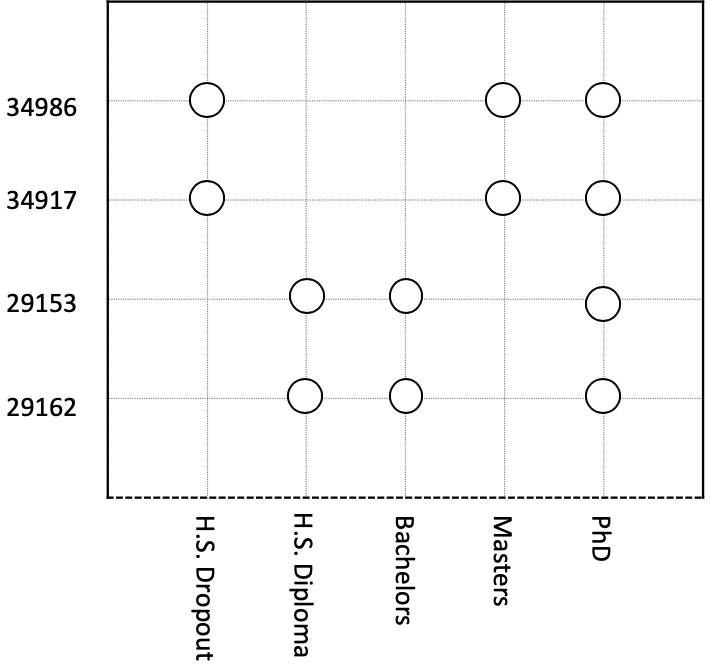
\includegraphics[scale=0.5]{background/fig/mondrian0.png}
    }
    \subfigure[First cut]{
        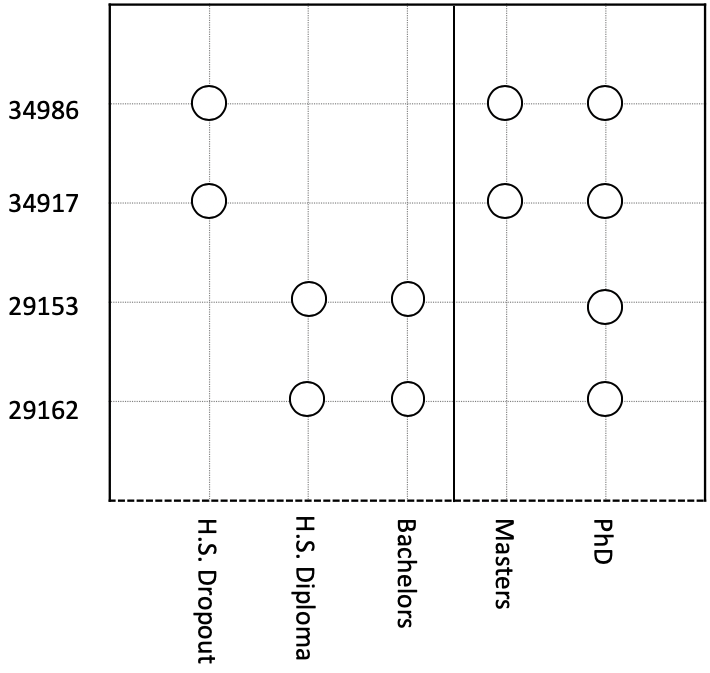
\includegraphics[scale=0.5]{background/fig/mondrian1.png}
    }
    \subfigure[Second cuts]{
        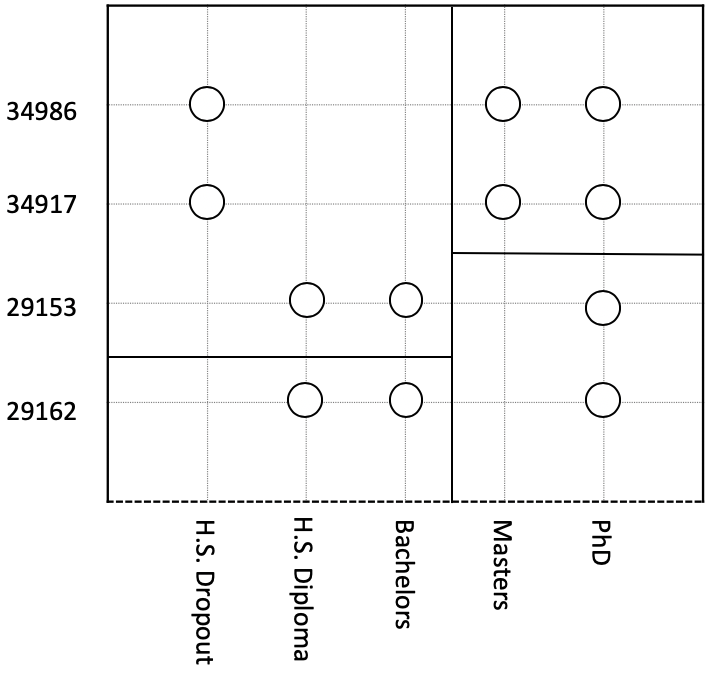
\includegraphics[scale=0.5]{background/fig/mondrian2.png}
    }
    \subfigure[Third and final cuts]{
        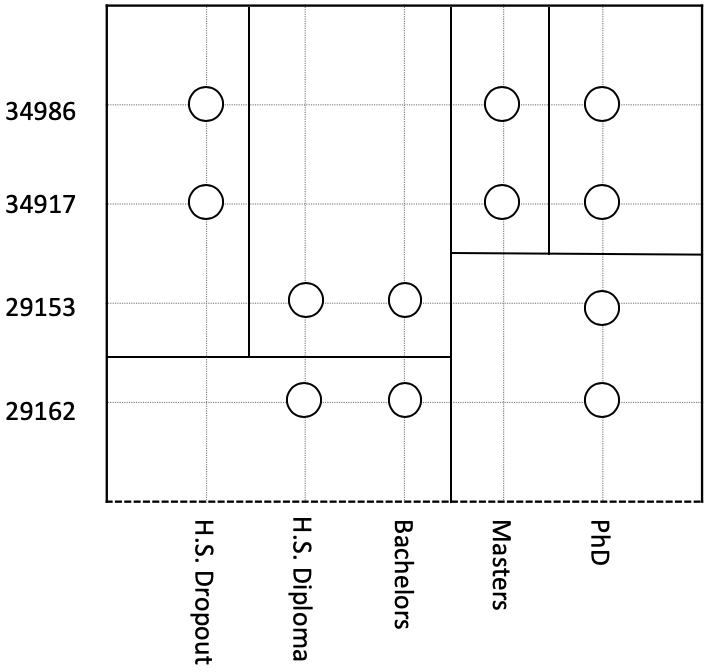
\includegraphics[scale=0.5]{background/fig/mondrian3.png}
    }
    \caption{A Figure representing the four steps in an example Mondrian $2$-anonymizing dataset containing two quasi-identifier, education level and zipcode. (a) is a 2D visualization of the two attributes. In (b), we show the first cut, separating the datapoints in two, along the axis with the largest normalized range of values. In (c), we see two additional cuts on the subsets, this time along the zipcode axis. Finally, the third cuts in (d) reveal the final regions for this Mondrian algorithm. We cannot go further otherwise we break the $k$ constraint.}
    \label{fig:mondrian_ex}
\end{figure}

Additionally, Mondrian has the additional flexibility of making DGHs for every quasi-identifier optional. Every region is bounded, and these can serve as generalization. Any numerical attribute has a clear lower and upper bound. In the absence of a DGH for the example in Figure \ref{fig:mondrian_ex}, the generalization examples we saw in \eqref{mondrian_gen1} and \eqref{mondrian_gen2} could have been as shown in \eqref{mondrian_no_dgh1} and \eqref{mondrian_no_dgh2}.

\begin{multline}
    \{(\mbox{H.S Dropout}, 34986), (\mbox{H.S Dropout}, 34917)\} \mapsto \\
    \{(\mbox{H.S. Dropout}, [34917-34986]),(\mbox{H.S. Dropout},
    [34917-34986]) \}
    \label{mondrian_no_dgh1}
\end{multline}
\begin{multline}
     \{(\mbox{Masters}, 34986), (\mbox{PhD}, 34986)\} \mapsto \{(\mbox{Masters -- PhD}, 34986), (\mbox{Masters -- PhD}, 34986)\}
     \label{mondrian_no_dgh2}
\end{multline}

The only caveat is for categorical attributes: they need to have a total ordering. Otherwise the notion of distance does not exist. For example, in Figure \ref{fig:mondrian_ex}, the distance between zipcodes is straightforward as it's a numerical attribute but the distances separating levels of education are abstract and have to be chosen. This can sometimes be a problem when the order isn't as clear, like a dataset including the Profession attribute with ground domain $\mbox{Prof}_0 = $\{Tech-support, Salesman, Skydiver, Farmer\}. There's no obvious order on which to base these which complicates the partitioning. 



\subsection{k-Anonymization Weaknesses}
We'd be remiss not to address the fact that k-Anonymization on its own is not a sufficient privacy measure. There are plenty of ways to work around the anonymization method like homogeneity attacks\cite{ldiversity} or skewness attacks \cite{critique_kanon}. Furthermore, private data holders have to be careful when releasing the same set anonymized in different ways as sometimes the tables can be relinked, and then de-anonymized\cite{kanon_orig}.

To counter some attacks, additional privacy measures have been introduced. For example, \textit{l-diversity} ensures that within every equivalence class at least $l$ different values are represented to counter homogeneity attacks \cite{ldiversity}. Similarly, \textit{t-closeness} verifies that the distribution of sensitive values in equivalence classes match the distribution of the sensitive values in the overall dataset to prevent an attacker from "learning too much individual-specific information"\cite{tcloseness}.

\section{Information Loss Metrics}
\label{sec:metrics}
When given a dataset to $k$-anonymize, the number of ways to do it grows exponentially with the number of quasi-identifiers. For example, every combination of VGHs for the quasi-identifiers will lead to a different anonymization. Additionally, the choice of algorithm will affect the results, as will the value of k.

Every different anonymization will thus lead to different amounts and types of lost information. Therefore, researchers have introduced Information Loss Metrics as a way to assess how $k$-anonymizations have affected the datasets and to try and capture how much information was lost in the process.

In all the metrics defined below, we $k$-anonymize a dataset $D$ to $D'$. The metrics are computed over the $m$ quasi-identifiers of $D'$. We denote cells in the original dataset as $a_{ij}$, and as $x_{ij}$ in the anonymized dataset. We also assume that a $DGH_j = \left(A_j, A_j^{(1)}, \dots, A_j^{(k_i)} = \{\varnothing\}\right)$ and associated $VGH_j = \left(\phi_j^{(1)}, \dots, \phi_j^{(k_j)}\right)$ are defined for each attribute $c_j$. 
Let $k_{ij}$ the depth of cell $x_{ij}$, the number of generalizations needed to obtain $x_{ij}$ from $a_{ij}$.
We further define for this VGH the reverse mapping: $\Phi^{-1}_{ij}(x_{ij}) = (\phi_{j}^{(1)})^{-1}\circ\dots\circ(\phi_{j}^{(k_{ij})})^{-1}(x_{ij}) \subseteq A_j$, as the set of all values $a \in A_j$ that could be anonymized to $x_{ij}$ through generalization. 

\subsection{Hierachy Based Metrics: Precision Metric}
\label{metrics_prec}
First, we try to quantify how generalized a table is. When working with DGHs, this can be done by taking into account how many times attributes are generalized (i.e., what depth of their DGH we've used):

Sweeney and Samarati first introduce the notion of distance to describe the level of generalization of a table with respect to other generalizations of the same table, based on single dimension generalization hierarchies \cite{distance_metrics}. We can quantify the absolute distance as follows:

$$
\mbox{Absolute Distance}(D, D') = \sum_{i=1}^m k_i
\label{abs_dist}
$$

Where $k_i$ represents the depth of generalization for attribute $i$. Nevertheless, this metric has the drawback of penalizing every generalization equally, whereas that may not be the case. For example, generalizing an attribute with a DGH of depth 1 will immediately suppress the column but will account for the same distance as a small generalization on an attribute with a deep DGH. 
For that reason, Sweeney and Samarati then described Relative Distance \cite{kanon_algos}. Relative Distance takes into account the depth of every DGH as well:

$$
    \mbox{Relative Distance}(D, D') = \sum_{i=1}^m \frac{k_i}{|DGH_i|}
    \label{rel_dist}
$$

This metric gives every attribute a score between 0, and 1. The former indicating an ungeneralized column, and the latter a full suppression. Given these two distance metrics, we can start quantifying data loss in single dimensional generalization algorithms. Nevertheless, this is still a broad metric as it is over an entire column. we can find more precise results by analyzing datasets at the cellular level.

Sweeney does this by defining precision \cite{kanon_algos}: a metric quantifying the distortion at cell level, defined as follows:

$$
    \mbox{Precision}(D, D') = 1 - \frac{\sum\limits_{i=1}^{|T|} \sum\limits_{j=1}^m \displaystyle\frac{k_{ij}}{|DGH_{i}|}} {m|D|}
    \label{precision}
$$

This takes the sum of the generalization level of every cell, and then normalizes it. This will return values between 0 and 1, from no generalization to full suppression. Subtracting this from 1, we get a metric determining the percentage of the table that is generalized. This metric is used to obtain minimal distortion in the MinGen algorithm (\nameref{mingen}), and we could use this to measure data degradation in algorithms with domain hierarchies.

Nevertheless, precision is a crude measure of degradation as different generalizations affect the data differently. Additionally, it relies on the DGHs created by the analyst. This has the downside of making it impossible to compare two generalizations created using different hierarchies, and a metric that can only be used in hierarchy-based models. Furthermore, we have no way to evaluate the DGHs themselves, making this entire metric dependent on the assumption that they're well defined.

\subsection{Entropy Metric}
Entropy, as defined by Shannon in 1948 in the context of his information theory research, is a measure to quantify information \cite{shannon_entropy}. In 2007, Gionis et al. started using it to assess the amount of information lost during an anonymization process \cite{entropy_measure}. More precisely, Gionis uses the conditional entropy $H(Y|X)$, quantifying the amount of information needed to describe needed to describe the outcome of a random variable $Y$, given the outcome of a random variable $X$. To understand how much information is lost, we want to find the conditional entropy of every cell in the generalized table with regards to the original table.

Let $x_{ij}$ a cell in $D'$, after some number $1 \leq k_{ij} \leq k_j$ of generalizations $x_{ij} \in A_j^{(k_{ij})}$. Let $V_{ij} = \Phi_{ij}^{-1}(x_{ij})$ be the set of all values that this cell could take in $D$. The entropy of that cell is defined as:
$$
    H(x_{ij}) = - \sum_{v \in V_{ij}} P(a_{ij} = v | x_{ij})\log P(a_{ij} = v | x_{ij})
$$
where $P(a_{ij}=v|x_{ij})$ describes the probability that $a_{ij}$, the original cell in $D$, is equal to $v$, given that the cell has value $x_{ij}$ in $D'$. It is computed from $D$ as:
$$
    P(a_{ij} = v|x_{ij}) = \frac{|\{1 \leq i \leq N: a_{ij}=v\}|}{|\{1 \leq i \leq N: a_{ij} \in V_{ij}\}|}
$$

The entropy of a dataset $D'$ is defined as the total entropy of its cells:
$$\Pi_e(D,D') = \sum\limits_{i=1}^{|T|} \sum\limits_{j=1}^{m} H(x_{ij})$$


The higher $\Pi_e$, the higher the conditional entropy, and the more data would be needed to describe what was lost. Nevertheless, it is hard to ensure what high entropy entails, or whether it is a good measure for utility.

\subsection{Classification Metric}
This metric, defined by Iyengar in 2002, has the aim of quantifying utility of a dataset to be used in classification tasks \cite{cm_granularity_metric}. When a dataset is k-anonymized, we would ideally want all the elements of an equivalence class to have the same class label. This would imply that the anonymization was, to some extent, justified in grouping these records together. Iyengar describes his metric as "[penalizing] impure groups"; equivalence classes that have been grouped although they represent different things.

This metric iterates through the records of an k-anonymized table $D'$, and penalizes every row who's class label is not the same as the majority label in its equivalence class:

$$
    CM(D') = \sum_{t \in D'} \frac{\mbox{penalty}(t)}{|D'|}
$$

Where the penalty is defined per equivalence class. Every class, through a majority vote, gets assigned a majority class label. Minority class records are penalized:

$$
    \mbox{penalty}(t) = 
    \begin{cases}
        1, & \text{if $D$ is suppressed}\\
        1, & \text{if class$(t) \not =$ class$(eq(t))$} \\
        0, & \text{otherwise}
    \end{cases}
$$

This metric essentially returns the maximum possible accuracy of a classifier on this dataset because every tuple in an equivalence class will get the same result, and assuming the classifier picks predicts the most prevalent label in the class, there will still be an error of the minority label. Intuitively, it also gives a measure of coherence of the anonymization, considering equivalent tuples should be under the same label.

\subsection{Discernibility Metric}
The discernibility metric was introduced by Bayardo in an attempt to capture information loss based on the sizes of equivalence classes \cite{discern_metric} : 
$$
discernibility(D') = \sum_{e \in eq(D')}|e|^2
$$
This metric sums the square of the equivalence class sizes. The justification is that the bigger the equivalence classes are, the more tuples will have to have been generalized to fit in broader categories and the more information will have been lost.

\subsection{Average Class Size Metric}
Similar to the Discernibility Metric, this metric takes into account equivalence class sizes to calculate utility \cite{mondrian}: 
$$
    C_{avg}(D') = \frac{|D'|}{k|eq(D')|}
$$
By taking into account $k$, this metric gives us an idea of how much larger the equivalence classes are than in the best case scenario, in which every equivalence class contains $k$ records. Compared to the Discernibility metric, this one is less punishing of large equivalence classes. However, it gives a more intuitive number than discernibility.

\subsection{Diameter Metric}
The diameter metric calculates the maximum Hamming distance between two records: 
$$
    diameter(D') = \max_{u, v \in D'}d(u,v)
$$
where  $d(u,v) = |\{j: u[j] \not= v[j]\}|$ \cite{meyerson2004complexity}. This metric can be used to quantify information loss because anonymous records all converge to the same suppressed values, thus, distances between records decrease the more they are generalized. Nevertheless, it's not very precise as it only uses Hamming distance, meaning it would give the same diameter to two points that are very similar but slightly different for every dimension as it would to two diametrically opposed points in the space. 



\subsection{Ambiguity Metric}
The ambiguity between dataset $D$ and its $k$-anonymous version $D'$ is defined as the average number of records that an anonymous record could represent in the original version \cite{ambiguity_metric}: 
$$
    Ambiguity(D,D') = \frac{1}{|D|} \sum_{i=1}^{|D|}\prod_{j=1}^{m}|\Phi^{-1}_{ij}(x_{ij})|
$$
As records are more generalized, ambiguity increases as the set of records it could represent grows. As such, we can use it to measure how much information has been lost through generalization. The limitation is that it doesn't account for distance within the attribute. For example, if a lot of values in a very small range are generalized to the same coarse point, then they'll have a high ambiguity metric, even if in the end not much information is lost. However, if two points that are far away are forced to generalize together then that is worse in terms of information loss but the metric will only recognize that the anonymous record could be one of two values, and will give it a better score.

\subsection{Granularity Metric}
The granularity of a dataset is defined as the fraction of values from the ground domain that an anonymous cell could possibly have been, other than its actual value \cite{cm_granularity_metric}:
$$
    granularity(D') = \sum_{i=1}^{|D'|} \sum_{j=1}^{m} \frac{\left|\Phi^{-1}_{ij}(x_{ij})\right| - 1}{|A_j|}
$$

Granularity is similar to Ambiguity, except at the cell level rather than record level. It has the same limitation of not taking into account distance between the grouped values. 

\subsection{Squared Distance Error Metric}
This metric takes the sum of distances between a record in the original table, and their counterpart in the anonymous table. Because anonymous records are either representative of ranges, or multiple values, we define their position as the average of the values it can take \cite{dse_metric}: 
$$
    E(x_{ij})= \frac{1}{|\Phi_{ij}^{-1}(x_{ij})|} \sum_{a \in \Phi_{ij}^{-1}(x_{ij})} a
$$
We can now take the sum Euclidean distances on the records between $D$ and $D'$:
$$
    Squared Distance Error(D, D')= \sum_{i=1}^{|D|} \sqrt{\sum_{j=1}^{m} (a_{ij}- E(x_{ij}))^2}
$$
This can help gauge how different the averages of the records, hence their values, are from the original value and helps give an idea of how much the information has changed. The downside with this metric is that compared to a metric like ambiguity, in which you know exactly what the result means-- the average fraction of original records representable by an anonymous record--, this one seems a bit more arbitrary.

\subsection{Information Loss Metric}
The Information Loss Metric is one that aims to simplify measuring loss of information in datasets that have a mixed of ordered and unordered attributes. Let $Ord$ be the attributes in $D$ that are ordered, and $UnOrd$ the unordered ones. We define this metric as \cite{ilm}: 
$$
    IL(e) = |e|\left(\sum_{j \in Ord}\frac{e_{j,max} - e_{j,min}}{|A_j|}
    + \sum_{j \in Unord}\frac{k_{ij}}{k_j}\right)
$$
For ordered values, we look at the fraction of values from the ground domain that are encompassed in this cell, and for unordered attribute, we take the depth of the value in that equivalence class.

The metric is then defined as the sum of $IL(e)$ over all equivalence classes of $D'$.

\subsection{Hellinger Metric}
The Hellinger Metric measures the distances between the quasi-identifier distribution of values before and after the $k$-anonymization. By taking the median value of the distances, we hope to get a representation of the entire dataset's anonymization qualities \cite{hellinger&biv}:
$$
    Hellinger(D,D') = \text{median}_j\left( d_{hell}(P_j,Q_j)\right)
$$

Where $P_j$, and $Q_j$, are the distributions of the values of attribute $j$ in $D$, and $D'$ respectively. $d_{hell}$ is the Hellinger distance between distributions:
$$
    hellinger(P,Q) = \frac{1}{\sqrt{2}}\sqrt{\sum_{i=1}^k(p(i) - q(i))^2}
$$
Similarly to the squared distance error metric, it's hard to interpret the value given for this metric. It's not immediately clear what hellinger distances entail in terms of utility.


\subsection{Bivariate Correlation Metric}
The Bivariate Correlation Metric compares the correlation between every pair of quasi-identifier in $D$, and $D'$, and measures the changes, returning the median value \cite{hellinger&biv}:

$$biv\_corr(D,D') = \text{median}_{j_1\neq j_2}\left(|V(j_1,j_2) - V(j'_1,j'_2)|\right)$$

For categorical attributes, we calculate correlation using Cramér's V: $V(j_1, j_2)$ the Cramér coefficient between columns $j_1$ and $j_2$ in the original dataset and $j'_1$, $j'_2$ the same columns in the anonymized dataset. Plagued by the same affliction as the other metrics that measure a distance, we do not have a clear idea of how to interpret these results. What distance becomes unacceptable in terms of utility? Or what does taking the median really do for us?

\chapter{Experiment: the Use of Information Loss Metrics as Utility Predictors}
Although information loss metrics are widely used as proxies to measure utility, there is no evidence they are as predictive as claimed. For that reason, we propose, and carry out, an experiment to determine their use in predicting the utility of $k$-anonymous datasets on classification tasks. We $k$-anonymize the same 4 datasets with many different anonymization hyperparameters (algorithm, VGHs, choice of k), looking at overall trends, and finding out whether the information loss metrics can accurately predict utility.


\section{Overview}
The aim of this experiment is to see if information loss metrics can predict the utility of a $k$-anonymous dataset, and we break the major components into a workflow depicted in Figure \ref{fig:workflow}

\begin{figure}[h]
    \centering
    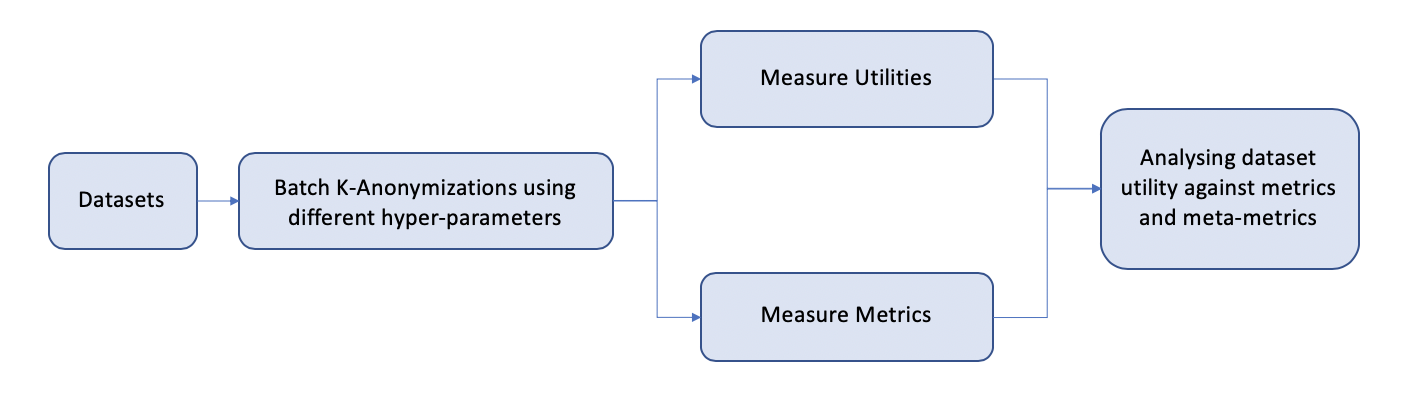
\includegraphics[width=\textwidth]{project/fig/overview.png}
    \caption{A representation of the experiment workflow. For a specific dataset, we create many different $k$-anonymous versions. For these anonymous datasets, we measure utility and the information loss metrics independently. With that information in hand, we try to make sense of it.}
    \label{fig:workflow}
\end{figure}

We start by picking four datasets that encompass a range of types of attributes and sizes. For each of these datasets, we create $600$ different $k$-anonymous versions of them, using different hyper-parameters. If information loss metrics can be used to predict utility, then, when we calculate said metrics for every anonymous dataset, and measure the datasets' utilities separately, we should be able to find some type of correlation. We use the performances of off-the-shelf classifiers trained on our anonymous datasets as a measure of utility, and avoid as much data processing on the $k$-anonymous sets as possible to remove any external influences.

Below, we explain the experimental setup for the different components involved:

\section{Datasets}
We analyze four different datasets, aiming to capture a large range of features, types, and sizes. All datasets are appropriate for classification tasks. In these datasets, the class label attribute is considered the sensitive attribute. All other attributes are quasi-identifiers.
\begin{itemize}
    \item \textbf{BIRTH} \cite{birth_dataset}: A national Indonesian survey on women’s contraceptive method of choice. It contains 1473 records and 9 quasi-identifiers, all ordinal. The sensitive attribute is the contraceptive method used (3 classes, moderately unbalanced). 
    \item \textbf{RING} \cite{ringnorm_dataset}: A synthetic dataset with points sampled from two 20-dimensional Gaussians. The first distribution has a mean of $0$ and a covariance of 4 times the identity; the second distribution has a mean of $(a,...,a)$, with $a=2/\sqrt{20}$, and a unit covariance. It contains 7400 rows and 20 continuous attributed. The sensitive attribute is the distribution from which the record was sampled (2 classes, balanced).
    \item \textbf{ADULT} \cite{adult_dataset}: Widely cited, Adult contains a slice of the results from the 1994 US Census data. Its associated classification task is predicting if an individual's salary is above or under 50k a year (our sensitive attribute). Removing records with missing entries, it contains $30,162$ rows and includes 3 ordinal, 2 continuous, and 7 unordered quasi-identifiers (2 classes, unbalanced).
    \item \textbf{HEART} \cite{heart_dataset}: A medical dataset for patients at risk of contracting a cardio vascular disease. It contains 4238 records and 15 attributes, a mix of ordinal and continuous (2 classes, heavily unbalanced).
\end{itemize}


\section{Anonymization}


\subsection{Algorithms Used}
While multiple algorithms have been proposed to achieve k-anonymity~\cite{incognito,kanon_algos,mondrian,ola_algo,arx}, we focus on two popular algorithms with an open source implementation, Datafly~\cite{kanon_algos} and Mondrian~\cite{mondrian}, using UTDallas' Anonymization Toolbox for the implementation of both algorithms \cite{utd_toolbox}. Additionally, we motivate a variant of a Datafly algorithm that removes order constraints on the attributes, thus allowing for more flexible generalization trees.

\begin{itemize}
    \item \textbf{Datafly}: For each quasi-identifier, we create a random generalization tree that respects attribute order (only adjacent attributes can be aggregated together). This variety in the generalization trees should result in datasets with differing utilities as some generalization trees will make more sense than others or preserve different pieces of information.
    
    \item \textbf{Datafly-Shuffled}: Same procedure as Datafly but removing the order constraint on the generalization tree. Intuitively, these trees ``break'' the ordinality of attibutes, and should make them less useful. Figure \ref{fig:shuffled_vgh_example} depicts an example of a possible VGH that respects order and would be used in the normal Datafly algorithm (VGH (a)), and one that could be used in a Datafly-Shuffled in which order is not respected (VGH (b)). We create this variant of Datafly to test the metrics' ability to recognise what will definitely turn into pointless anonymous datasets. We expect some metric to be unable to spot the difference, particularly those that only quantify information loss without taking into account features of the data, like Entropy.
    
    \item \textbf{Mondrian}: Mondrian assumes that all data is ordinal, and uses multi-dimensional local generalization algorithms to generalize close records together. In order to generate many random datasets, we randomly permute the values of attributes, keeping the data semantically identical but breaking the natural ordering of values. Permutations that keep a logical order are more likely to offer coherent results whereas permutations that groups values nonsensically will be less useful.
\end{itemize}

For every algorithm, we discretize continuous attributes by binning them into 20 buckets, each containing 5\% of the range of the data. When dealing with unordered attributes like Nationality, or Profession, we randomize their order, no matter the algorithm. We generate 200 $k$-anonymous versions of every dataset, for every algorithm. 


%Normal vs Shuffled VGH
\begin{figure}
\centering
\subfigure[VGH, respecting order]{
    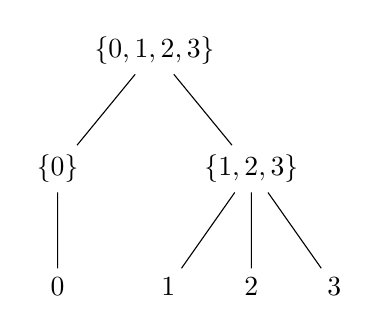
\begin{tikzpicture}[sibling distance=7em,
    level 2/.style={sibling distance=3em}]]
    \node {$\{0,1,2,3\}$} 
        child { node {$\{0\}$}
            child { node {$0$}}
        }
        child { node {$\{1,2,3\}$}
            child { node {$1$}}
            child { node {$2$}}
            child { node {$3$}}
        }
    ;
    \end{tikzpicture}}
\hspace{2cm}
\subfigure[VGH, unordered]{
    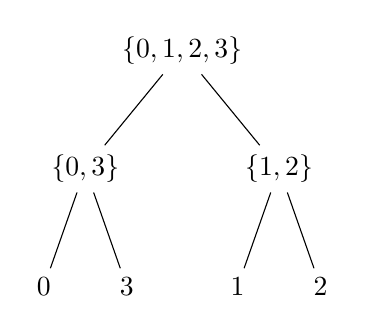
\begin{tikzpicture}[sibling distance=7em,
    level 2/.style={sibling distance=3em}]]
    \node {$\{0,1,2,3\}$} 
        child { node {$\{0,3\}$}
            child { node {$0$}}
            child { node {$3$}}
        }
        child { node {$\{1,2\}$}
            child { node {$1$}}
            child { node {$2$}}
        }
    ;
    \end{tikzpicture}}
\caption{Two example of possible VGHs on a categorical attribute with 4 possible values. The left-hand-side VGH respects order; the right-hand-side VGH does not}
\label{fig:shuffled_vgh_example}
\end{figure}


\subsection{VGH Creation}
To create random VGHs, we use sets to represent the generalization levels. For example, a cell with value $\{0,1,2,3\}$ could have any of the elements in the set as an original value.

The procedure is as follows:
\begin{enumerate}
    \item We start with a full set of the domain ground values. This represents the fully suppressed value at the top of the generalization tree.
    \item We split this set into an ordered partition-- a partition in which values still appear in increasing order.
    \item We recursively keep on splitting the subsets of the partitions, until we reach a singleton elements, representing the ground domain values. 
\end{enumerate}

This returns a tree of values, with ground values as leaves, with a generalization for every step up the tree. However, we have an additional constraint: every leaf node needs to be at the same depth. This is because Datafly performs global single-dimensional generalizations and we thus need coherence between the generalization levels of values within an attribute. As such, we find the shallowest leaf node in our tree, and prune any branch that extends past that by setting all the elements in the parent node as individual leaves. Figure \ref{fig:vgh_creation} displays an example of a possible generalization tree creation before we insert the depth constraint, and after. 

\begin{figure}
\centering
\subfigure[VGH, no depth constraint]{
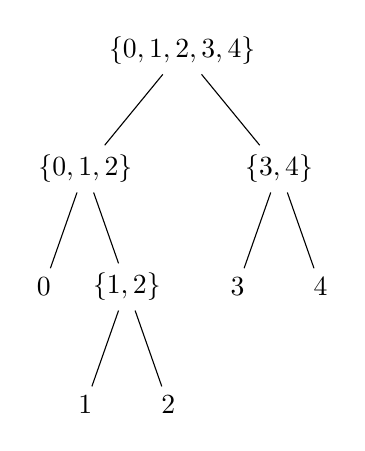
\begin{tikzpicture}[sibling distance=7em,
    level 2/.style={sibling distance=3em},
    level 3/.style={sibling distance=3em}]]
    \node {$\{0,1,2,3,4\}$} 
        child { node {$\{0,1,2\}$}
            child { node {$0$}}
            child { node {\{$1,2$\}}
                child {node {$1$}}
                child {node {$2$}}
            }
        }
        child { node {$\{3,4\}$}
            child { node {$3$}}
            child { node {$4$}}
        }
    ;
    \end{tikzpicture}}
\hspace{2cm}
\subfigure[VGH, with depth constraint]{
    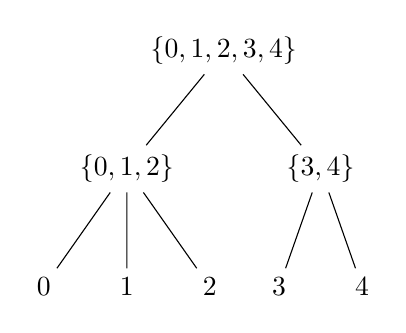
\begin{tikzpicture}[sibling distance=7em,
    level 2/.style={sibling distance=3em},
    level 3/.style={sibling distance=3em}]]
    \node {$\{0,1,2,3,4\}$} 
        child { node {$\{0,1,2\}$}
            child { node {$0$}}
            child { node {$1$}}
            child { node {$2$}}
        }
        child { node {$\{3,4\}$}
            child { node {$3$}}
            child { node {$4$}}
        }
    ;
    \end{tikzpicture}}
\caption{An example of how a generalization tree randomly created for a 5-valued attribute, and how that tree looks when respecting the depth constraint. The shallowest leaf in VGH (a) occurs at depth 2 so we turn the set $\{1,2\}$ into two separate leaves, and prune any branch extending deeper}
\label{fig:vgh_creation}
\end{figure}

\subsection{Choice of k}
An initial exploration revealed that an increasing $k$ value quickly destroyed the dataset, and, ultimately, led to noisy, nearly random classification results, with very little utility for a classification task. We show this in Figure \ref{fig:varying_k_birth_mondrian_knn} for a Mondrian algorithm on the Birth dataset using a k-Nearest Neighbour Classifier. We see a slight decreasing trend in utility until around the $k=20$ mark, after which the results, become very noisy but seem to have very little utility, as judged by the dashed black line representing the accuracy baseline.

\begin{figure}
    \centerfloat
    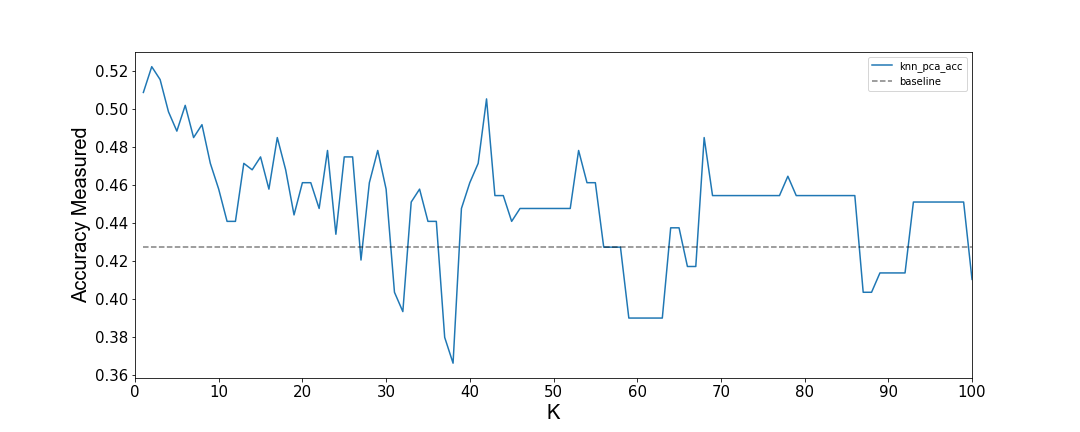
\includegraphics[width=1.2\textwidth]{project/fig/varying_k_birth_mondrian_knn.png}
    \caption{Plot of the measured accuracy (blue) and a baseline accuracy for a k-Nearest Neighbour Classifier trained on a Mondrian $k$-anonymous birth dataset with increasing $k$ values. The dashed black line represents the accuracy baseline. The results show an initial steep decrease in accuracy (i.e., utility) that flattens out quickly. For values larger than $k=20$, we assume the varying results are noise.}
    \label{fig:varying_k_birth_mondrian_knn}
\end{figure}

Because the most significant data destruction happens for small values of $k$, we restrict our $k$ parameter choice to small values. Nevertheless, we found that fixing $k=2$ could restrict the range of some metrics. In an attempt to add some flexibility, we set the k parameters of the 200 datasets to samples from $k = X + 2$, where $X \sim Poi(1)$. This guarantees small $k \geq 2$ values, but also grants a larger range for the information loss metrics.

\section{Machine Learning Tasks}
\subsection{Pre-Processing Anonymous Datasets}
After the anonymization, we need a way to format the results so we can use them in our classification tasks. They cannot be left as a single range per attribute because there are unordered shuffled attributes that could potentially lead to disjoint sets of possible original values. We choose a solution akin to one-hotting: we turn every record into binary tuples of possible original values. Take a cell $x_{ij}$ from an anonymous record, representing a set of values. For the set of values in attribute $A_j$, $\{a_j^{(1)},...,a_j^{(l)}\}$, we turn anonymous cell $x_{ij}$ into a binary tuple of size $l$, defined as follows: 

$$t_{ij} = (1 \mbox{ if } a_j^{(k)} \in x_{ij} \mbox{ else } 0)_{k=1}^l$$

We rebuild records by concatenating the tuples for all attributes.

As an example, take the dataset with attributes Age, categorically ranging from $0$ to $3$, and Gender, a binary choice, in Table \ref{tab:bitmap_example}. This method allows for arbitrary sets of numbers, and can thus be used for all our algorithms.

\begin{figure}
\centering
\subfigure[$D'$, a $2$-anonymous dataset]{
    \begin{tabular}{|l|l|}
        \hline
        Gender & Age \\
        \hline
        \{0\} & \{1,3\}  \\
        \{0\} & \{1,3\}  \\
        \{0, 1\} & \{0,1\}  \\
        \{0, 1\} & \{0,1\}  \\
        \hline
    \end{tabular}}
\subfigure[D', as a concatenation of tuples]{
\begin{tabular}{|l|l|l|l|l|l|}
\hline
gender\_0 & gender\_1 & age\_0 & age\_1 & age\_2 & age\_3\\
\hline
1 & 0 & 0 & 1 & 0 & 1 \\
1 & 0 & 0 & 1 & 0 & 1 \\
1 & 1 & 1 & 1 & 0 & 0 \\
1 & 1 & 1 & 1 & 0 & 0 \\
\hline
\end{tabular}}
\caption{An example to show a transformation between cells containing sets of values for age and gender attributes into binary tuples representing the same information}
\label{tab:bitmap_example}
\end{figure}

We apply the same process to the original data, essentially one-hotting it.

\subsection{Classifiers and Utility Measures}
\label{sec:util_measures}
For this project, we use our $k$-anonymous datasets as training sets for off-the-shelf classifiers and test their performance on the original test data. We equate a dataset's utility to the obtained performances when used as a training set.

To reduce the risk of measuring metric utilities that will be entirely dependent on the classifier used, we train three types of classifiers for every dataset, and measure both accuracy, and the Area Under the Receiver operating characteristic (AUROC). The three types of classifiers are as follow: 

\begin{itemize}
    \item Logistic Regression
    \item Random Forest after Principal Component Analysis (PCA) transformation with .95 explained variance
    \item K-Nearest Neighbours after PCA transformation with .95 explained variance
\end{itemize}
Although the idea was to keep the anonymous data manipulation to a strict minimum, avoiding any external factors that could affect measured utility, the number of columns after turning records into binary arrays was such that the Curse of Dimensionality became an issue. Therefore, we add a PCA transformation to the two classifiers most sensitive to this problem. Additionally, the datasets were so destroyed by the anonymization process-- most columns would be fully suppressed--  that an explained variance of $0.95$ could usually be reached in very few dimensions, making k-NN and RF classifiers simple and intuitive choices.

This method of measuring utility results in 600 different $k$-anonymous versions of every dataset (200 for each algorithm used), with six different measures of utility.



\section{Metrics Used}
We implement all the metrics described in the Information Loss Metrics section (\ref{sec:metrics}) apart from Precision. This is because the metric takes into account the anonymous dataset's DGHs' depths and would require us to extend the definition of this metric for the Mondrian anonymizations, in which the concept of depth is inapplicable. To keep the experiment constant over all the algorithms, we decide to forego Precision.

These metrics were chosen because they were either presented with the purpose of measuring utility, or because they have been used as utility predictors in the literature and/or industry.

We design our experiment to scale every metric into the range $[0,1]$. Some metrics occur in this range by definition, like the Classification Metric. For the others, we divide the result by the worse possible case metric: we take a fully suppressed version of the dataset, and calculate the metric of that dataset.


\section{Meta-Metric}
\label{sec:metametrics}
The results, found in Chapter \ref{chap:results}, imply very little correlation between information loss metrics and dataset utility. Nevertheless, we do not reach a definite conclusion because the claim that metrics reflect utility is difficulty falsifiable-- the metrics might very well reflect utility except that we simply do not understand how to use them correctly. 

Instead, we propose a secondary analysis: if, when given all the metrics, we can train a regressive model that correctly predicts utility in datasets, then the metrics must have some predictive power. Here, we try to emulate the best case situation: our model will learn as much information as it can on all the combined metrics and the resulting measured utilities, and will therefore be able to make much deeper inferences than we could. Therefore, if the model can predict utility, then we must concede that somewhere in the metrics lies information about utility and that we just could not see it. However, if the model still cannot predict utility, then it must be that the metrics are not viable because even a model trained on the task could not draw the link between them.

We design our Regression model to take a dataset in which the features are our metrics, and every row represents a $k$-anonymous dataset on which we calculated the metrics. The target variable for a model will be one of the different utility measures we describe in Section \ref{sec:util_measures}. For every model, we take 10\% of our data as a testing set.

We use a library called auto-sklearn, an automated machine learning toolkit \cite{autosklearn}. Given a single parameter, running time, this library uses Bayesian optimization and meta-learning to construct an ensemble model for a regression task. This allows us to train regressors on our metrics impartially by giving each learning task the same amount of time to train: 24 hours. The resulting ensemble will be our best predictor at the potential accuracy of our test datasets and we coin it a Meta-Metric. 

We train an auto-sklearn model per utility measure, and per dataset. Furthermore, we need to separate the algorithms used. This is because, as seen in the scatterplots \ref{fig:metrics_scatter1} and \ref{fig:metrics_scatter2}, the metric results for Datafly algorithms are disjoint clusters from the Mondrian results (we explain further in Section \ref{sec:single_metrics}). This is a problem as any decent machine-learning task can distinguish between two separate clusters. Additionally, we know that Mondrian datasets tend to outperform Datafly datasets in the utility measures. Because of those disparities in both the utility measures, and the metrics, our model would only have to learn to differentiate between a Mondrian and Datafly algorithm to score well. However, this simplifies the task, and the algorithm used should be irrelevant. As such, the model will be a better predictor of utility than it should be because, instead of predicting the utility of the metrics, it will predict whether the dataset will have the utility of a Mondrian dataset, or a Datafly one.







\chapter{Results and Analysis}
\label{chap:results}
\section{Single Metrics}
\subsection{Scatterplots}
\label{sec:single_metrics}
We first visualize the results by plotting scatters of the metrics individually against the measured utility obtained by the different classifiers in Figures \ref{fig:metrics_scatter1}, and \ref{fig:metrics_scatter2}. This will help us get an idea of what to look at that and how to later quantify our findings. Every row represents a metric and columns are split between classifiers. Every scatterplot contains a line of best fit per dataset and the different datasets are separated by color. The gradient of these lines represent how changes in utility are reflected in the metrics. Broadly, we address the following: 
\begin{itemize}
    \item Per dataset, every metric tends to be separated into two disjoint point clusters, corresponding to the different algorithms
    \item For a metric, consistency, or lack thereof, across the datasets
    \item For a metric, consistency, or lack thereof, across the classifiers
    \item Some metrics have no linear correlation
\end{itemize}

These four points provide evidence for the limitations of individual metrics in predicting utility for $k$-anonymous datasets. Consistent trends are necessary for a metric to be useful because they represent how changes in utility are reflected in the metric. We need to be able to compare two different values for a metric and know what that difference in value implies for an arbitrary combination of dataset, algorithm, and classification task. The results show that we cannot do this with our metrics as we obtain inconsistent trends.

\begin{figure}
    \centerfloat
    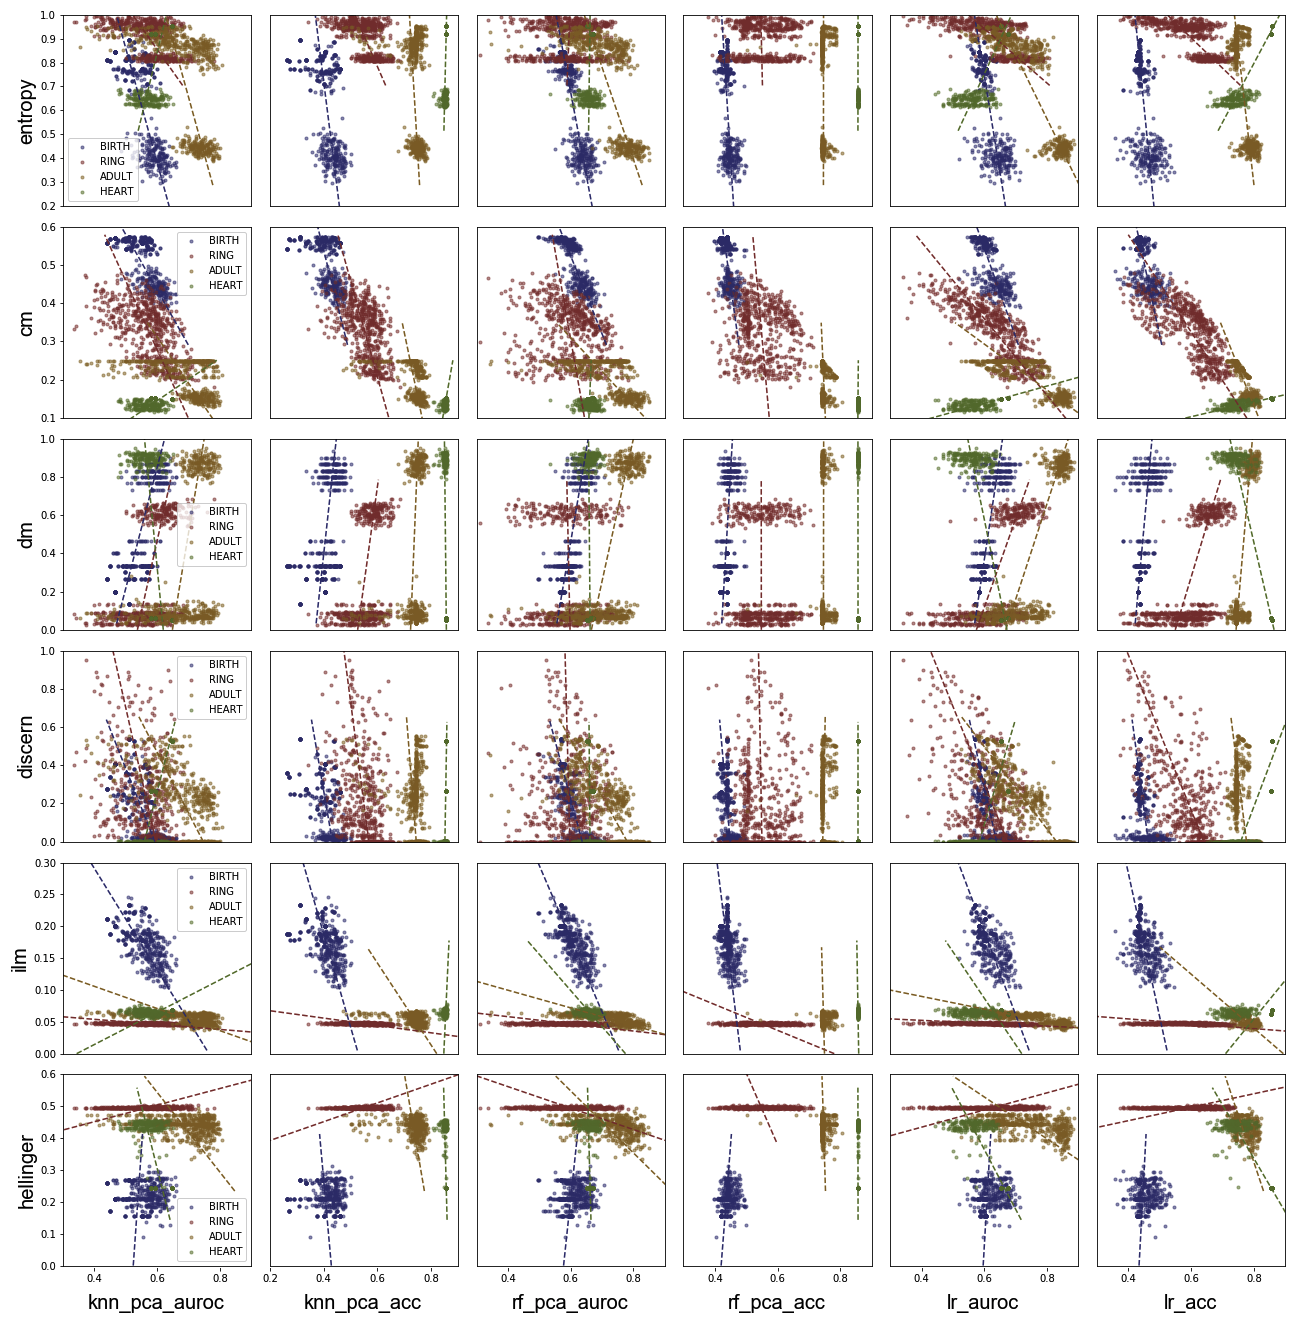
\includegraphics[width=1.2\textwidth]{project/fig/metrics-vs-accs_1.png}
    \caption{(Part 1) Scatterplots of the metrics against the classifiers for all datasets, separated by color. The dotted line is a line of best fit on a dataset obtained on all algorithms combined. We find separate clusters of points for every dataset caused by the difference in results for the different algorithms. Some metrics have consistent trends-- like the classification or diameter metrics -- across datasets, others, like the information loss metric, do not. We also look at the trends across classifiers used, and across the algorithms.}
    \label{fig:metrics_scatter1}
\end{figure}
\begin{figure}
    \centerfloat
    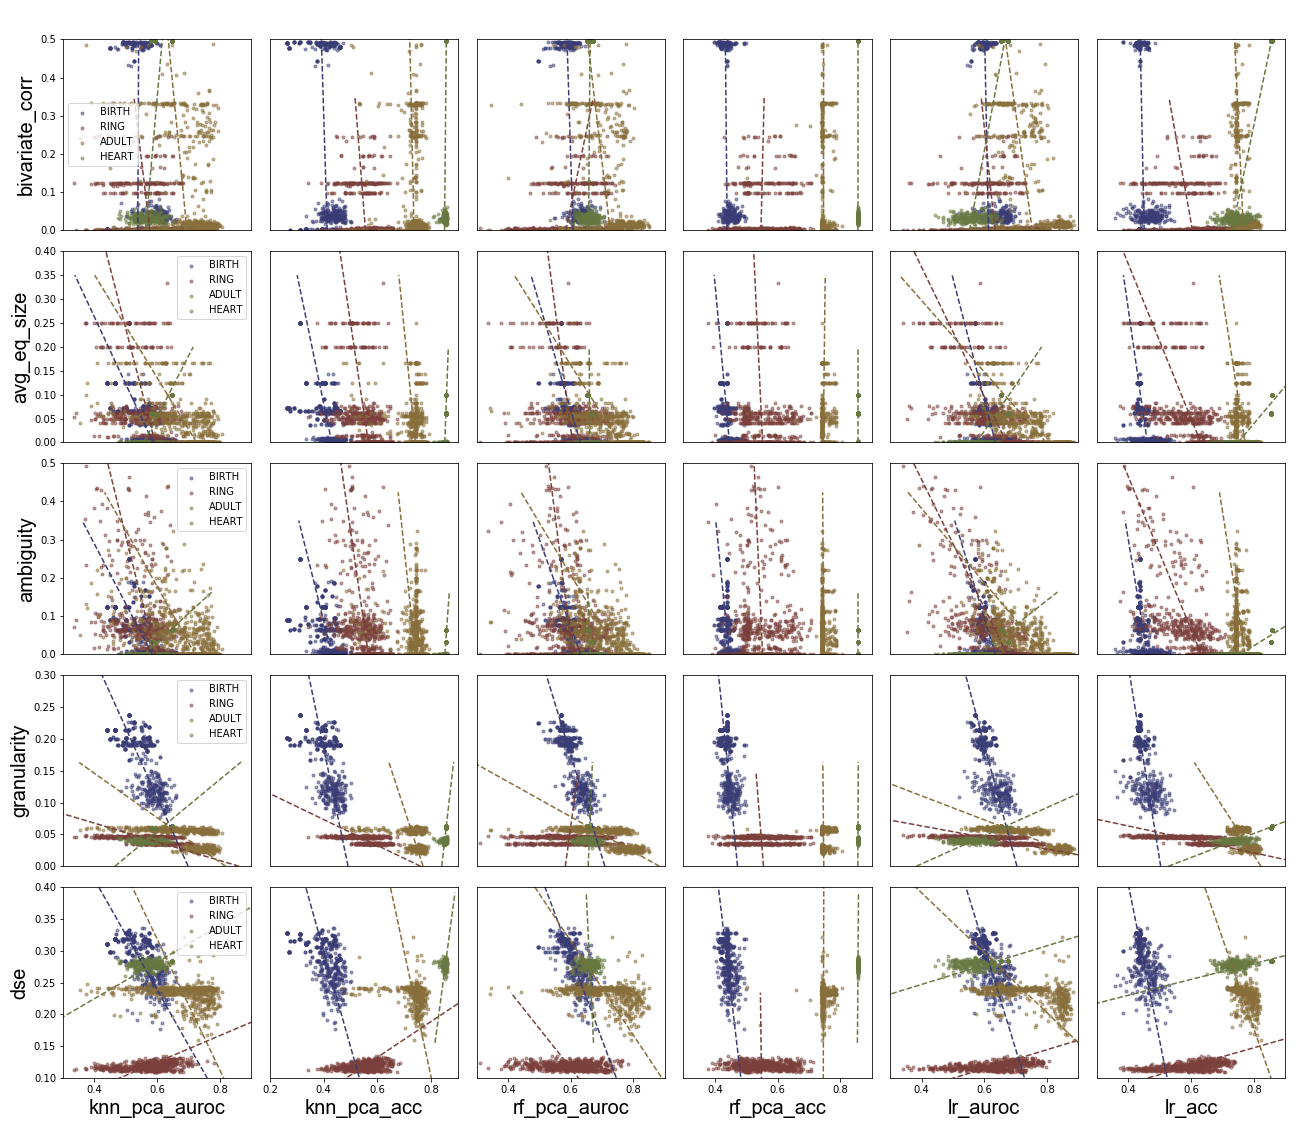
\includegraphics[width=1.2\textwidth]{project/fig/metrics-vs-accs_2.png}
    \caption{(Part 2) Scatterplots of the metrics against the classifiers for all datasets, separated by color. The dotted line is a line of best fit on a dataset obtained on all algorithms combined.}
    \label{fig:metrics_scatter2}
\end{figure}

\subsubsection{Disjoint Metric Clusters}
We first address the disjoint clusters found for every dataset: these are accounted for by the difference in algorithms. Mondrian outperforms the Datafly algorithms in terms of information preservation and this is reflected in the metrics. We can see the difference per algorithm more clearly in Figures \ref{fig:metric_hist1}, and \ref{fig:metric_hist2},  representing the distribution of metric results per algorithm used. 

In the metric distribution histograms mentioned above, we tend to see both Datafly algorithms heavily overlapping on their 200 respective datasets. While this is expected in metrics like \textbf{Entropy} that just quantify information loss, we do not spot major differences for metrics that actually look at the properties of the anonymous dataset-- the \textbf{Classification Metric}, for example. We would expect the equivalence classes in Datafly-Shuffled to have more diverse classification labels as we do not limit ourselves to grouping neighbouring, and thus similar, records. Nevertheless, we see that both Datafly algorithms are nearly overlapping, and so consistently across the datasets. This is unexpected as we designed the Datafly-Shuffled algorithm to intentionally lower its output's utility and it does not seem like it did.


\begin{figure}
    \centerfloat
    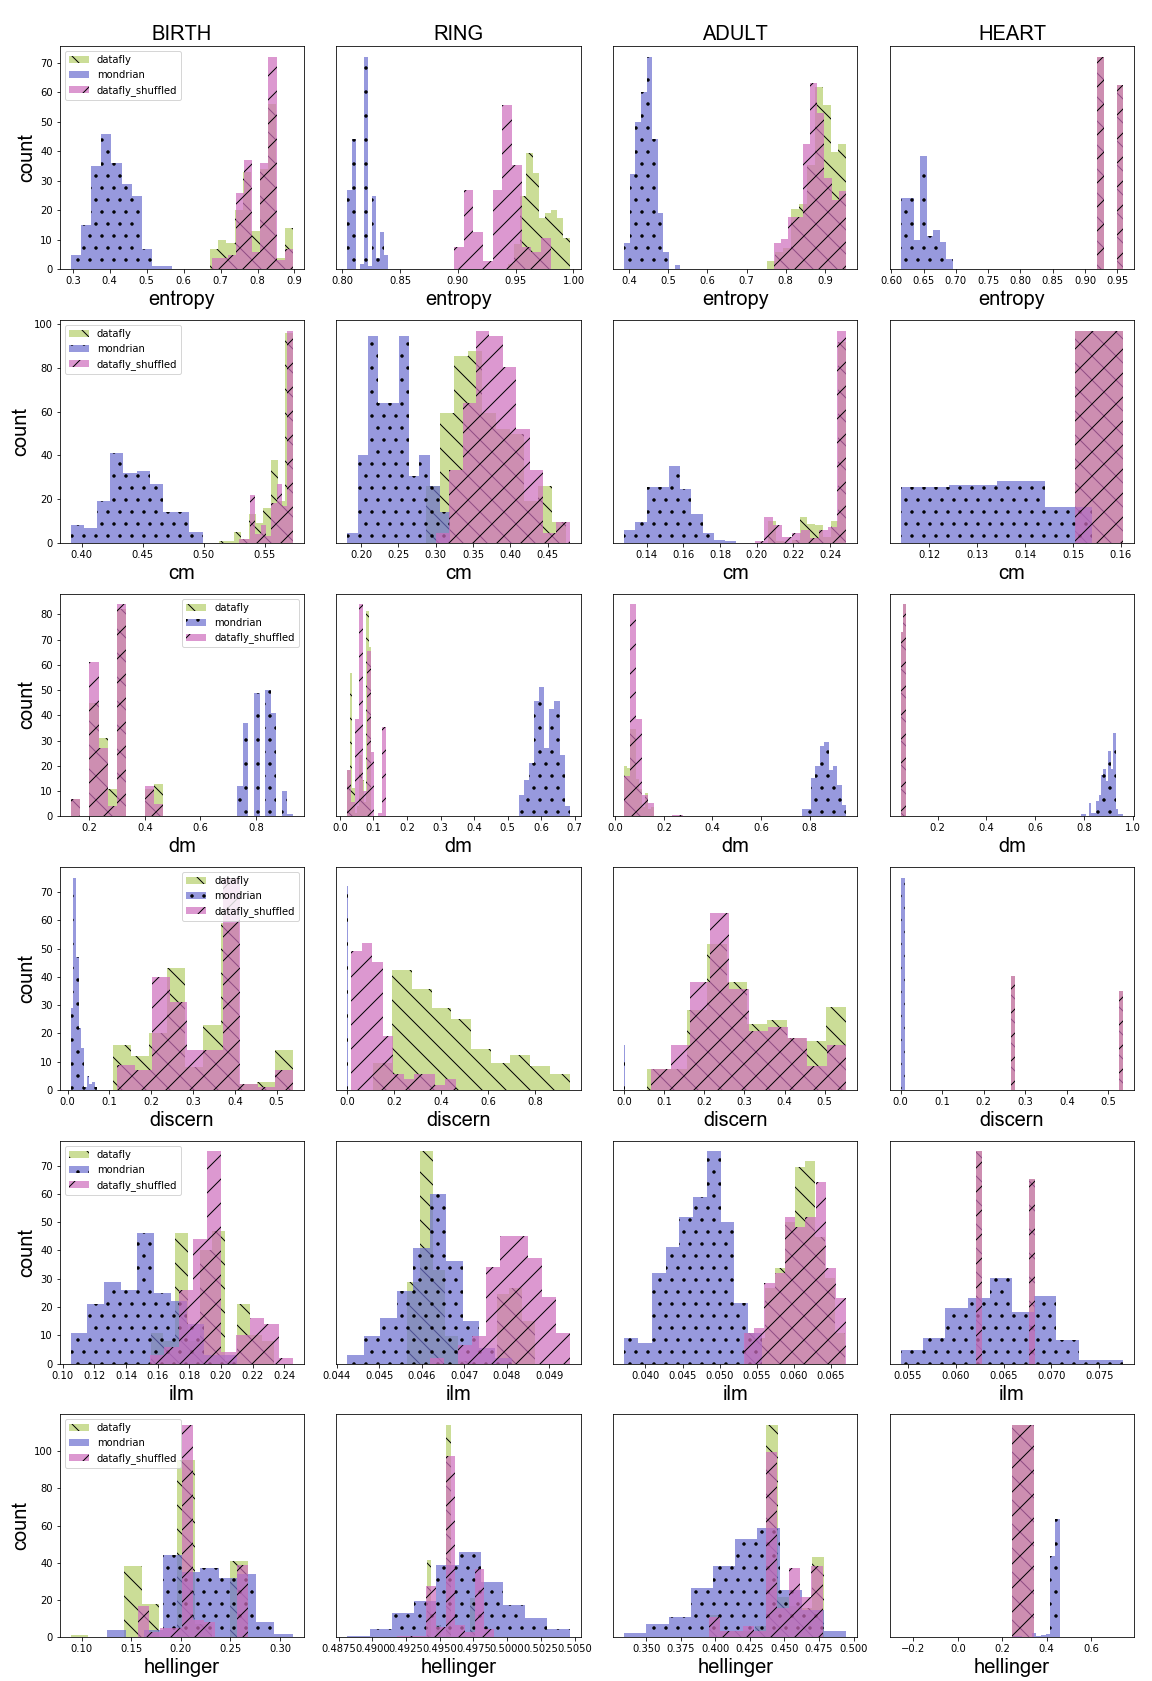
\includegraphics[width=\textwidth]{project/fig/metrics_hist_1.png}
    \caption{(Part 1) Histograms of the metrics over the four different datasets. The results show consistent overlap for the two Datafly algorithms while the Mondrian results stand apart.}
    \label{fig:metric_hist1}
\end{figure}
\begin{figure}
    \centerfloat
    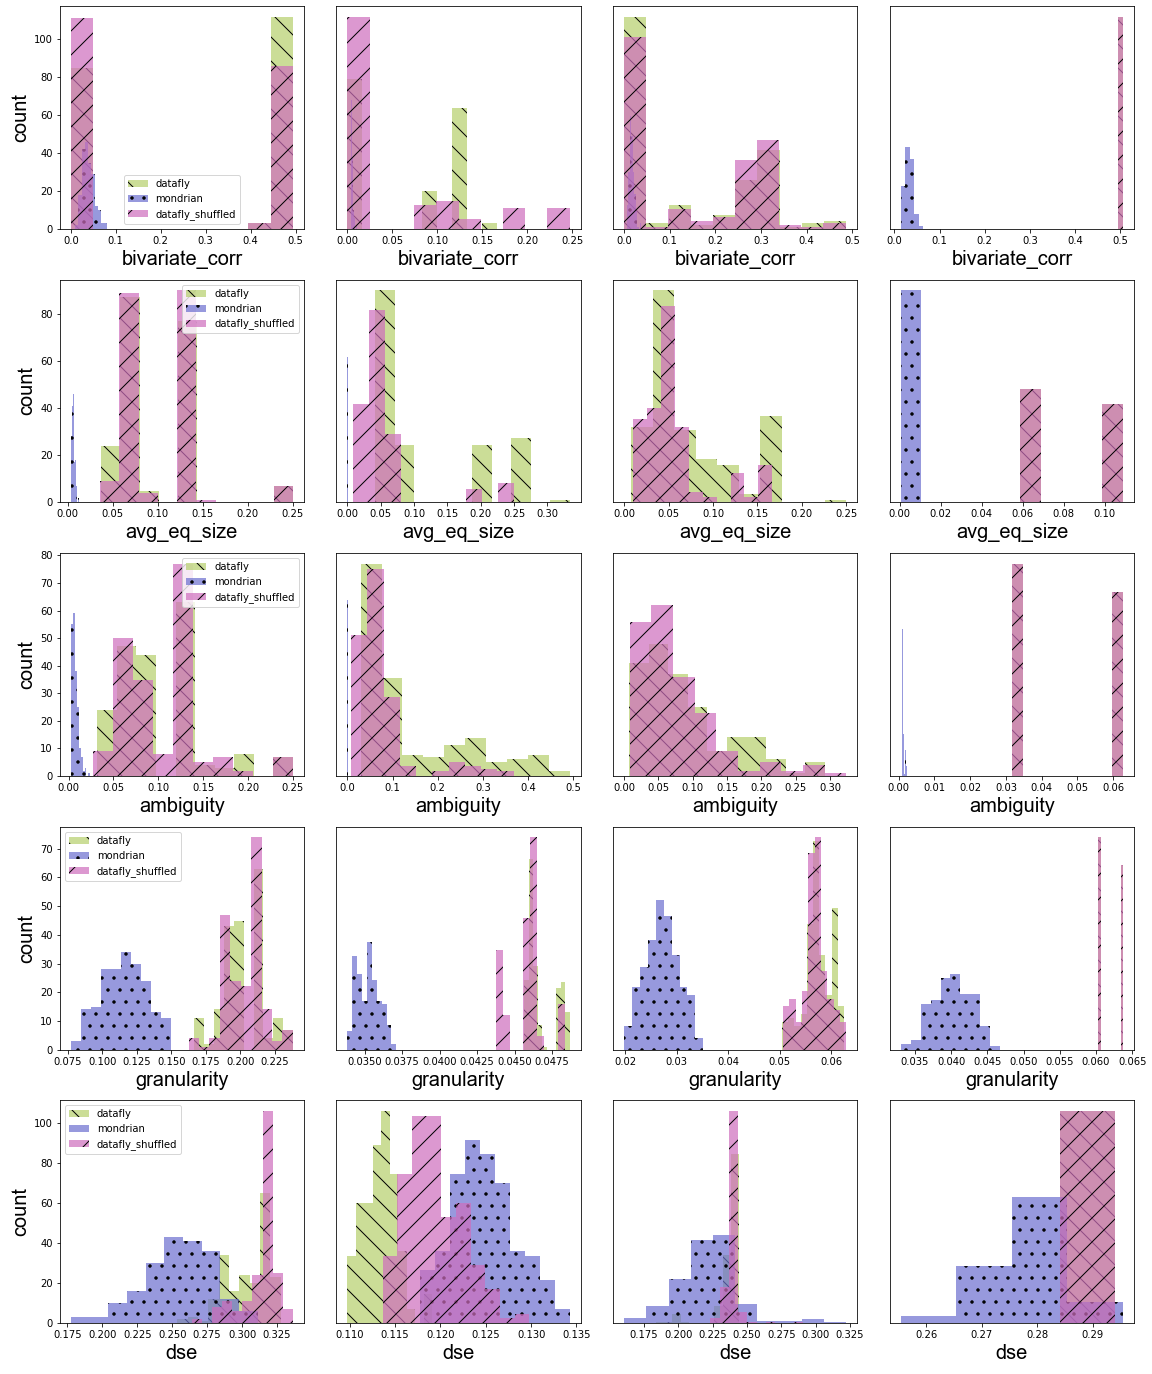
\includegraphics[width=\textwidth]{project/fig/metrics_hist_2.png}
    \caption{(Part 2) Histograms of the metrics over the four different datasets. The results show consistent overlap for the two Datafly algorithms while the Mondrian results stand apart.}
    \label{fig:metric_hist2}
\end{figure}

In Figure \ref{fig:hist_accs_perd}, we plot the distribution of the utility measures recorded on the different datasets and with the different algorithms. We observe that here, too, the Datafly-Shuffled datasets have very similar results to normal Dataflys datasets, allowing classifiers to perform equally well. The implication is that the classification metric did not differentiate between datasets of the two different algorithms because the two were inherently similar, and not because it is a bad metric.

The lack of difference in the shuffled and normal datafly datasets was surprising at first. Nevertheless, looking back at the datasets used, we found that this is due to the nature of the Datafly algorithm: it will generalize the attribute with the largest domain every time. Heuristically, this makes sense. However, it means binary attributes, like gender, are left untouched to the very end, due to their small ground domain size. All the while, the rest of the quasi-identifiers take heavy information losses. These binary attributes end up being the only non-suppressed values. On top of that, whether the binary attributes are switched or not is something any good classifier can work around. In short, the Datafly and Datafly-Shuffled datasets will tend to similar results because of how Datafly picks columns to generalize, and the fact it destroys most of the information that would create a difference between the modified algorithm and the original, even for small $k$ values, like $k=2$.

\begin{figure}
    \centerfloat
    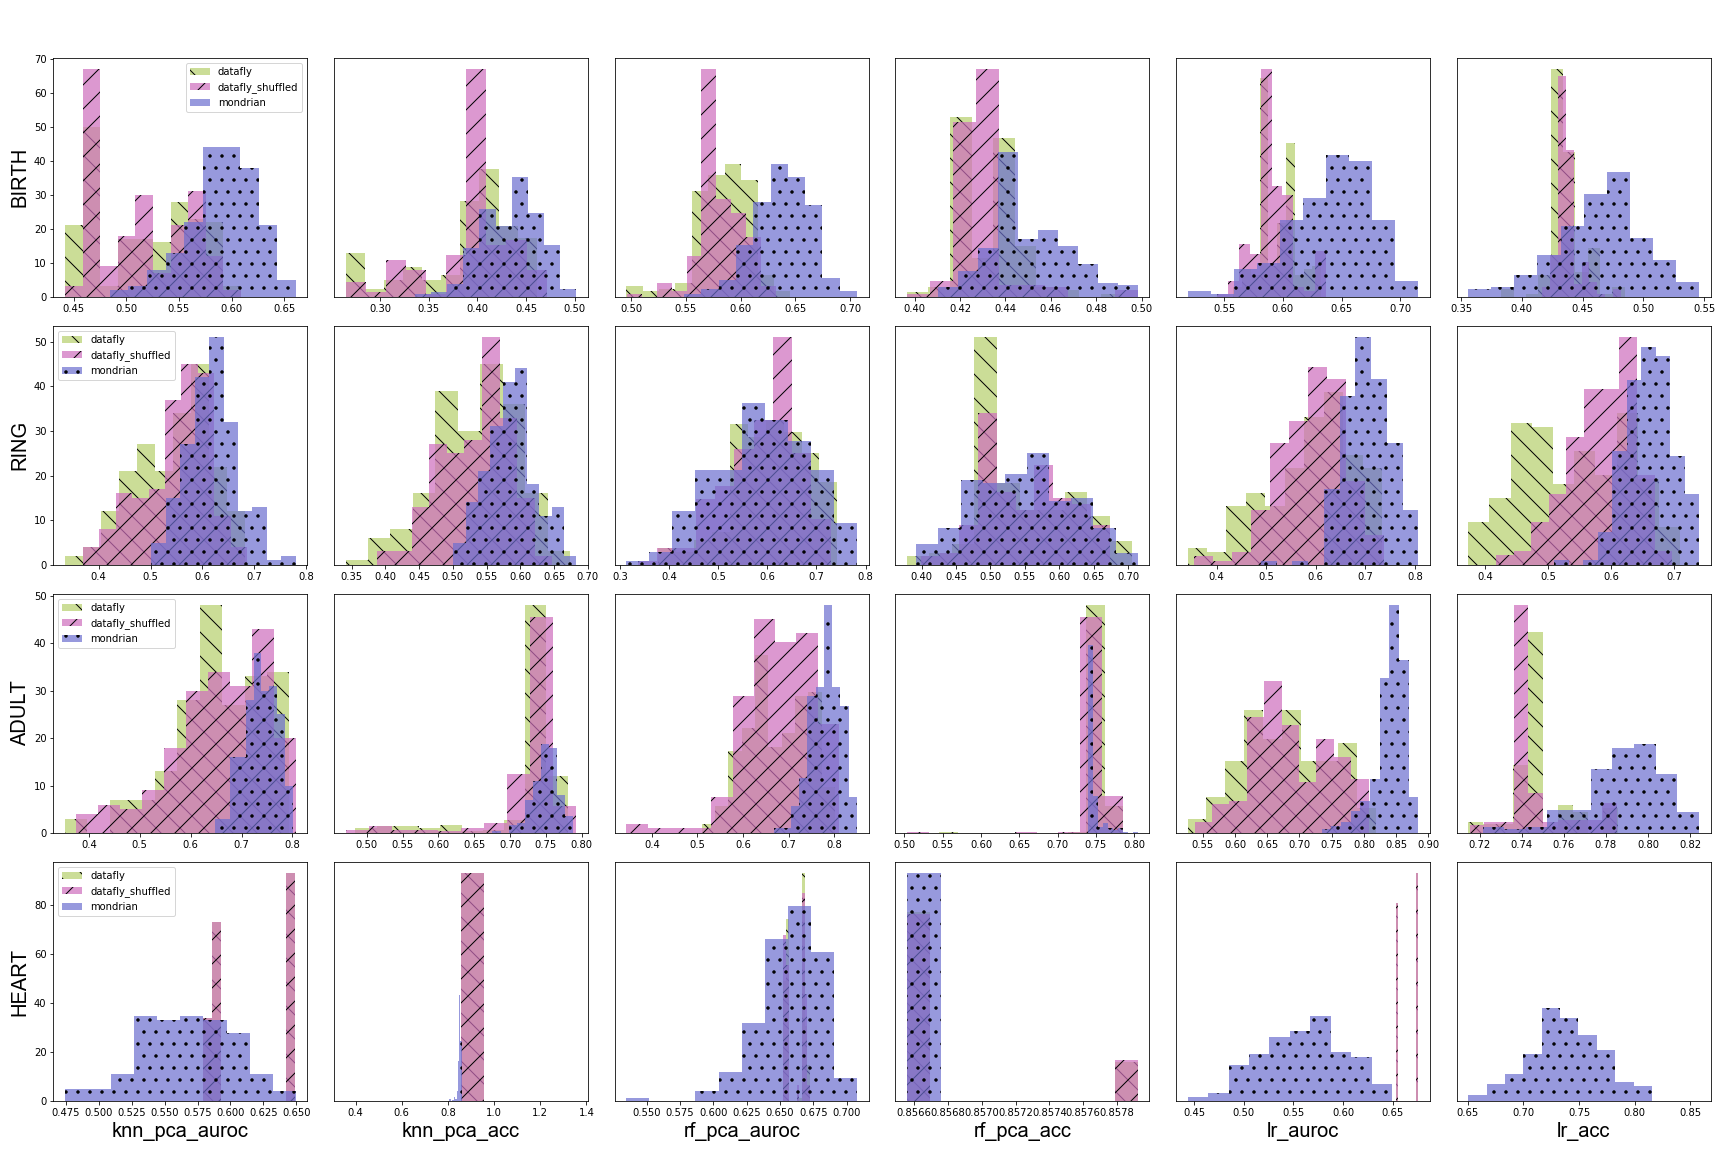
\includegraphics[width=1.2\textwidth]{project/fig/pat_full_accs.png}
    \caption{A set of histograms representing the distribution of measured utilities on different datasets (split by algorithm used). We see significant overlap on the two Datafly algorithms, and a tendancy for Mondrian datasets to score slightly higher than the others.}
    \label{fig:hist_accs_perd}
\end{figure}

\subsubsection{Trends for a Metric Across the Datasets}
\label{subsec:trends_datasets}
The metrics have varying success in getting consistent results across datasets. This can once again be seen in Figures \ref{fig:metrics_scatter1} and \ref{fig:metrics_scatter2}-- the scatterplots of the metrics for the different utility measures. 

Depending on the metric, when comparing the lines of best fits for the datasets in the same graphs, we get some mixed results. The \textbf{classification metric} manages to perform well: for all utility measures, all but the heart trend lines agree. Similarly so for the \textbf{diameter}, \textbf{average equivalence class size}, and a few other metrics. Nevertheless, the lines of best fit are not very pronounced (nearly vertical), implying little use for the metric: if, regardless of the metric score, we obtain the same utility, then the metric has zero predictive power. Other metrics do not do as well in terms of the consistency of their trends; the \textbf{hellingers}, \textbf{ilm}, and \textbf{squared distance error} metrics regularly have lines of best fit perpendicular to each other within the same graphs. This implies that even if a metric had predictive power on a dataset, it would be non-transferable to another, significantly reducing its real life applicability.

Furthermore, these trends are dataset wide and do not take into account the different algorithms. For example, looking at the \textbf{entropy} scatterplots (Fig. \ref{fig:metrics_scatter1}), we see the lines of best fit are influenced by having to connect the two disjoint clusters of different algorithms. If, instead, we fit a line per algorithm per dataset, we get Figures \ref{fig:sep_trends_gran} and \ref{fig:sep_trends_hell}, for the metrics of \textbf{granularity} and \textbf{hellinger}, respectively. For the sake of brevity, we do not include these figures for every metric, instead picking two good examples to illustrate this issue with the metrics. The full set of figures can be found in Appendix \ref{app:sep_trends_per_algo}. Notice that for the granularity metric (Fig. \ref{fig:sep_trends_gran}), lines of the same color (i.e., same dataset but different algorithms) are consistent; they have similar trajectories. 

However, when looking at the same plots for the \textbf{hellinger} metric (Fig. \ref{fig:sep_trends_hell}), we find a lot less consistency per dataset. For example, in the random forest accuracy plot (bottom, left), two out of the four datasets have nearly perpendicular trends on different algorithms. This occurs for most utility measures across this metric, particularly on the ring datasets (red).

\begin{figure}
    \centering
    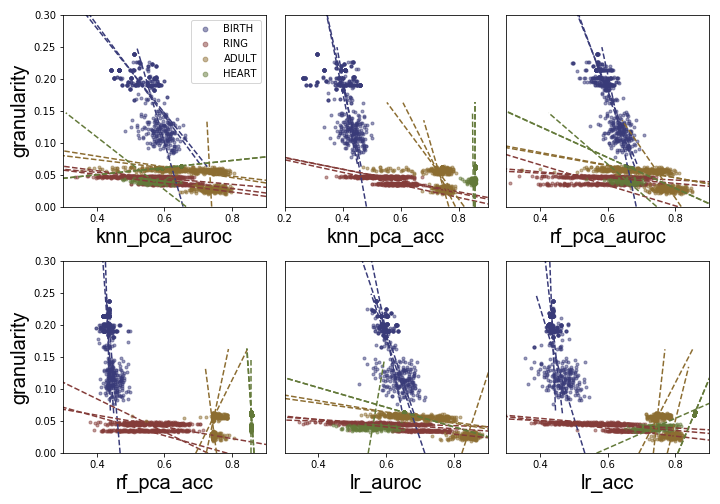
\includegraphics[width=0.8\textwidth]{project/fig/scatter_sep_trends/granularity_scatter.png}
    \caption{Scatterplots of the utility measures for the different classifiers against the granularity metric, separated by datasets. For every dataset, we draw a line of best fit per algorithm in order to show that lines for the different algorithms are consistent on the same datasets.}
    \label{fig:sep_trends_gran}
\end{figure}

\begin{figure}
    \centering
    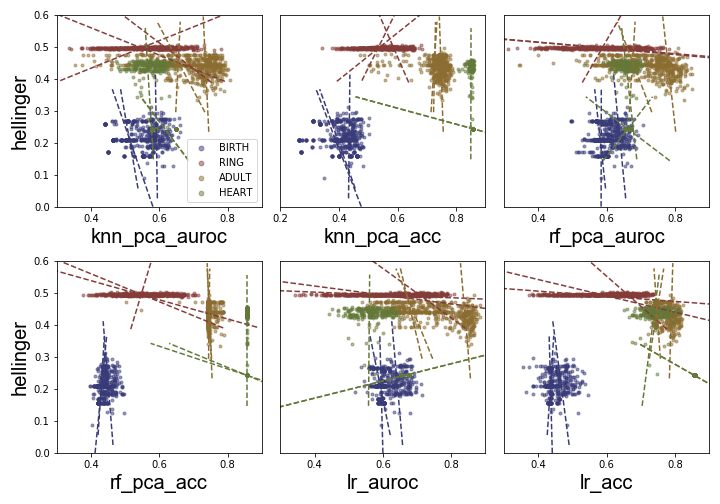
\includegraphics[width=0.8\textwidth]{project/fig/scatter_sep_trends/hellinger_scatter.png}
    \caption{Scatterplots of the utility measures for the different classifiers against the hellinger metric, separated by datasets. For every dataset, we draw a line of best fit per algorithm in order to show that lines for the different algorithms are \textbf{not} consistent on the same datasets.}
    \label{fig:sep_trends_hell}
\end{figure}

We mention this to highlight an issue with the metrics: their specificity-- we see that the trends are specific to the dataset, and furthermore, not all metrics are consistent based on the algorithm used. So, even starting from the hypothesis that metrics have some ability to predict dataset utility (which has not been convincing this far), before we could use metrics on a dataset, we would need to figure out what the trends are on that specific dataset. That means running experiments to figure it out, invalidating the whole point of metrics being an effortless way to predict utility.

\subsubsection{Trends for a Metric Across Classifiers}
Another dimension we can look at is whether the metric trends are consistent across the different classifiers and utility measures used. If this were the case, we could then argue that, at least, they have applicability irrespective of the classification task. We look at Figures \ref{fig:metrics_scatter1} and \ref{fig:metrics_scatter2} to compare the trends for the same datasets on different classification scores. For a metric to be useful, we need the trends for each dataset to be consistent across the row.

We find that the clearer the separation between the Datafly datasets and the Mondrian ones, the more consistent the lines of best fit are across the classifiers. For example, the \textbf{entropy} plots (Fig. \ref{fig:metrics_scatter1}, \ref{fig:metric_hist1}) show clear divisions between the metric results for Mondrian and Datafly results. This, in turn, forces the line of best fit to accommodate both sets of results and the larger the distance, the less variability we have in the slope of the best fit line. However, for metrics that have more overlap in the results for different algorithms-- like \textbf{Hellinger} (Fig. \ref{fig:metric_hist1}, \ref{fig:metrics_scatter1}), or \textbf{squared distance error} (Fig. \ref{fig:metric_hist2}, \ref{fig:metrics_scatter2}) metrics-- we find more variance in the lines of best fit. 

To remediate this, we create lines of best fit for the different algorithms. We refer, once again, to Figures \ref{fig:sep_trends_gran} and \ref{fig:sep_trends_hell}. These show that even though we have conditioned on the algorithm, we still have no consistency through the classification tasks. Looking at the \textbf{granularity} scatterplots (Fig. \ref{fig:sep_trends_gran}): the ring lines of best (red) fit stay consistent but because the metrics barely vary. We get some regularity for the birth datasets (blue), but very little for the adult dataset (yellow), alternating between positive and negative trends. We find equally erratic results on the \textbf{hellinger} metric scatters (Fig. \ref{fig:sep_trends_hell}), in which even the flat ring results (red) create lines of best fit seemingly randomly.


\subsubsection{No Linear Correlations}
We've mainly focused on the consistency of the lines of best fit throughout datasets/classifiers to test the applicability of metrics. Nevertheless, on top of consistency, we need the lines of best fit to contain some information. We find that a lot of trends that are very close to vertical, implying no linear correlation between the utility measures and metrics. For example, looking at metrics such as \textbf{bivariate correlation}, \textbf{diameter}, or \textbf{discernibility} in Figures \ref{fig:metrics_scatter1} and \ref{fig:metrics_scatter2} we find near vertical lines of best fit. In those cases, regardless of the metric score, the datasets have the same utility; it tells us nothing. Similarly, we find nearly horizontal lines for the ring dataset on information loss metrics: no matter the utility of a dataset, the metric spits out the same output, once again revealing nothing.


%\subsubsection{Summary of Scatterplots and Histograms}
%Through this section, we've seen that for a metric to be useful, it needs to be consistent no matter the dataset, the algorithm used, or the classification task. If it does not have these things, then it does not convey an interesting measure. On top of the consistency, it should also have some measure of correlation with the measured utilities, otherwise it has no value as a predictor.

%We find a few metrics that are relatively consistent through both the datasets, and the classifiers used: the classification, diameter, and average equivalence class size metrics. Nevertheless, we see the usefulness of the diameter metric drop because the trends are nearly vertical. The average equivalence class size has more pronounced trends, and so does the classification metric, although a lot more noisy.

%For most metrics, we double down on stating that they lack applicability due to their specificity. Based on what we've noted, if we wanted to use a metric to predict the utility of a dataset, we would need to do a lot of work to figure out the exact trend for the specific dataset being used. We would also need to ensure that the metric in question is consistent irrespective of the classifier used. To top it off, this is all based on the assumption that the metric has any predictive value, which isn't a given considering the metrics we've analyzed rarely fulfilled the criteria to be useful.

\subsection{Linear Regression: Metric Importance}
Using a different approach to assess the metrics, we attempt to find the most ``useful'' metric. We do this by fitting Linear Regressions on our standardized metrics, with the 6 model accuracies and AUROCs as the target variables. We consider the coefficients attributed to all the metrics. A larger coefficient implies a more significant impact on the regression, and, thus, more predictive power. Conditioning on the $k$-anonymization algorithm used and the dataset, we fit 72 linear regressions (4 datasets $\times$ 3 algorithms $\times$ 6 utility measures). 

For every metric, we measure the average effect size, and plot that in Figure \ref{fig:lin_reg}, along with the confidence intervals for these values. We find that the Average Class Size, Granularity, and Discernibility Metrics have the largest effect sizes. The Information Loss Metric is large too, but has an error margin that goes below most of the other metrics and their respective confidence intervals. The Hellinger, Bivariate Correlation, and Squared Distance Error are never the ones to have most added value.

Two metrics use the equivalence class sizes as a measure of utility: the Average Class Size Metric and the Discernibility Metric. The fact they both have large effect sizes indicate that equivalence classes are a good and easy way to assess a dataset's utility. Additionally, Average Class Size is amongst the metrics we recognized as potentially viable in the Single Metrics section, \ref{sec:single_metrics}.

Considering the way to measure utility was using classification tasks, it is surprising that the Classification Metric does not have larger effect sizes. It also had promising results in \ref{sec:single_metrics}. As a theoretical maximum measure, it might be that our classification tasks lacked the depth needed to achieve the optimal results, thus reducing the usefulness of the theory-based metric. 

The Hellinger, Bivariate Correlation, and Squared Distance Error Metrics bring up the rear in terms of largest average effect sizes. Hellinger and Bivariate, both presented by El Emam, et al., are ways to measure how the distributions of attributes change. This result might indicate that, in our usecase (i.e., a classification task), keeping attribute distributions constant is not a primary concern. Instead, based on the performance of the average equivalence class size, and discernibility metrics, we should shift our focus to how the records are grouped and generalized.

 
\begin{figure}[h]
    \centerfloat
    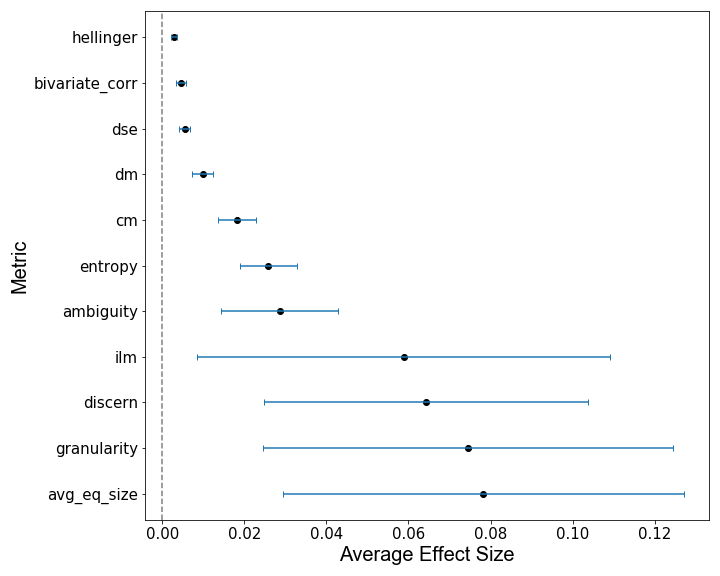
\includegraphics[width=0.8\textwidth]{project/fig/linreg_conf_interval.png}
    \caption{Fitting a linear regression on every utility measure, conditioned for dataset and algorithm, we measure the average effect size for the different metrics, along with the 0.95 confidence intervals. We find granularity, average equivalence class size, and discernibility to have higher effect sizes than the rest. However, their confidence intervals are equally large. Three metrics that measure distance, hellinger, bivariate correlation, and squared distance error, trail behind. All the confidence intervals are very large, but none pass over the $x=0$ line.}
    \label{fig:lin_reg}
\end{figure}


\subsection{1v1 Metric Prediction}
\label{sec:1v1_single}
As our analysis has been mostly qualitative in looking at the trends, we propose a more practical and quantitative way to test for a metric's use in predicting utility. The situation an analyst will often find themselves in is the following: given two $k$-anonymous datasets, which of the two should they use to maximize the utility? This will often happen when analysts use anonymization software like ARX \cite{arx}, for example. The platform allows you to easily modulate a few hyperparameters, and the actual anonymization is taken care of. The software outputs your anonymous dataset, and a list of metrics. 

In this case, the question becomes how much we should trust a metric, not based on a trend, but on a binary decision: we want to see how often, using a single metric, we can predict which dataset, out of two, has the most utility based on which has the best metric score. We then compare this to a baseline of a random choice, picking the best dataset 50\% of the time.

For every dataset and metric, we select $1000$ pairs of anonymous datasets in each algorithm used, and for every target utility measure. For every selected pair, we check if the dataset with the best metric score is also the one with the best utility measure. We then aggregate over the algorithm, and utility measures, to give a single rate per metric. 

%We condition on the algorithm because we notice that the metric results are always much better for the Mondrian datasets. Additionally, the Mondrian datasets generally outperform the Datafly sets as classification task training sets. Thus, if we compared a Mondrian to a Datafly, most of the time, it will have a better metric and a better utility. This is problematic as the metric comparison essentially turns into recognizing a Mondrian dataset from a Datafly one, a simpler task than predicting its utility. Instead, we look to compare identical algorithms only, averaging over the results.

\begin{table}
    \resizebox{\textwidth}{!}{%
    \begin{tabular}{|l|l|l|l|l|l|l|l|l|l|l|l|}
    \hline
    \rowcolor{gray!50}
    dataset & entropy & cm    & dm    & discern & ilm   & hellinger & bivariate\_corr & avg\_eq\_size & ambiguity & granularity & dse   \\ \hline
    \cellcolor{gray!50} birth   & 0.572   & 0.604 & 0.716 & 0.561   & 0.579 & 0.622     & 0.613           & 0.559         & 0.573     & 0.572       & 0.556 \\
    \cellcolor{gray!50} ring    & 0.593   & 0.644 & 0.591 & 0.587   & 0.604 & 0.621     & 0.573           & 0.562         & 0.599     & 0.605       & 0.554 \\
    \cellcolor{gray!50} adult   & 0.676   & 0.572 & 0.592 & 0.661   & 0.589 & 0.607     & 0.579           & 0.621         & 0.609     & 0.604       & 0.552 \\
    \cellcolor{gray!50} heart   & 0.752   & 0.774 & 0.768 & 0.747   & 0.748 & 0.872     & 0.728           & 0.748         & 0.748     & 0.75        & 0.742 \\ \hline
    \end{tabular}
    }
    \caption{A table displaying the rate of correctness when, comparing two $k$-anonymous datasets on a single metric, the anonymous dataset with the best metric score is also the one with the most utility. We see every metric predict at its best on the heart dataset, sometimes by large margins. Other than that, their predictive capacity is limited.}
    \label{tab:1v1_single_metrics}
\end{table}

We display the results in Table \ref{tab:1v1_single_metrics}. On the first three datasets (birth,ring,adult), the results are relatively similar-- scoring between 55.9\% and 71.6\%, and differing by a few percents inside the datasets. However, every metric predicts more accurately on the heart dataset than the others, correctly pointing to the dataset with the most utility around $75\%$ of the time. We believe this it might be due to the heavily unbalanced nature of the dataset. However, we merely offer it as a hypothesis as we have no proof to back it up.

Comparing the results to a random choice, we find the odds using metrics are better, but only marginally so.

This practical test provides a good place to wrap up the analysis of metrics individually. We have observed that metrics can separate a $k$-anonymous dataset anonymized using Mondrian from one anonymized with either of the Datafly algorithm. However, once the algorithm is fixed, no metric can consistently and successfully pick a dataset that has managed to retain more utility than other-- we only get a marginal increase in the probability of picking the correct one. As such, these metrics are not ideal tools to assess utility after a $k$-anonymization. Until an alternative is proposed, metrics could be used, but should always be taken with a grain of salt.


\section{Meta-Metrics}
As described in section \ref{sec:metametrics}, we aim to show that even tapping their full potential, metrics are only so predictive. We train a Meta-Metric-- an Auto-Sklearn ensemble model-- per combination of dataset, algorithm, and utility measure. We then use a test set of metrics to measure the accuracy of our Meta-Metric in predicting the utility of a dataset. We plot the Meta-Metrics' predicted utilities against the real measured utility as scatterplots on the different datasets and utility measures in Figure \ref{fig:meta_scatter}. Every color represents the Meta-Metric for a specific algorithm. The results show that most of the Meta-Metrics are good utility predictors because the trend lines are regularly close to the reference $y=x$ line. We generally find good trends but noisy results. 

%Normal Scatter
\begin{figure}
    \centerfloat
    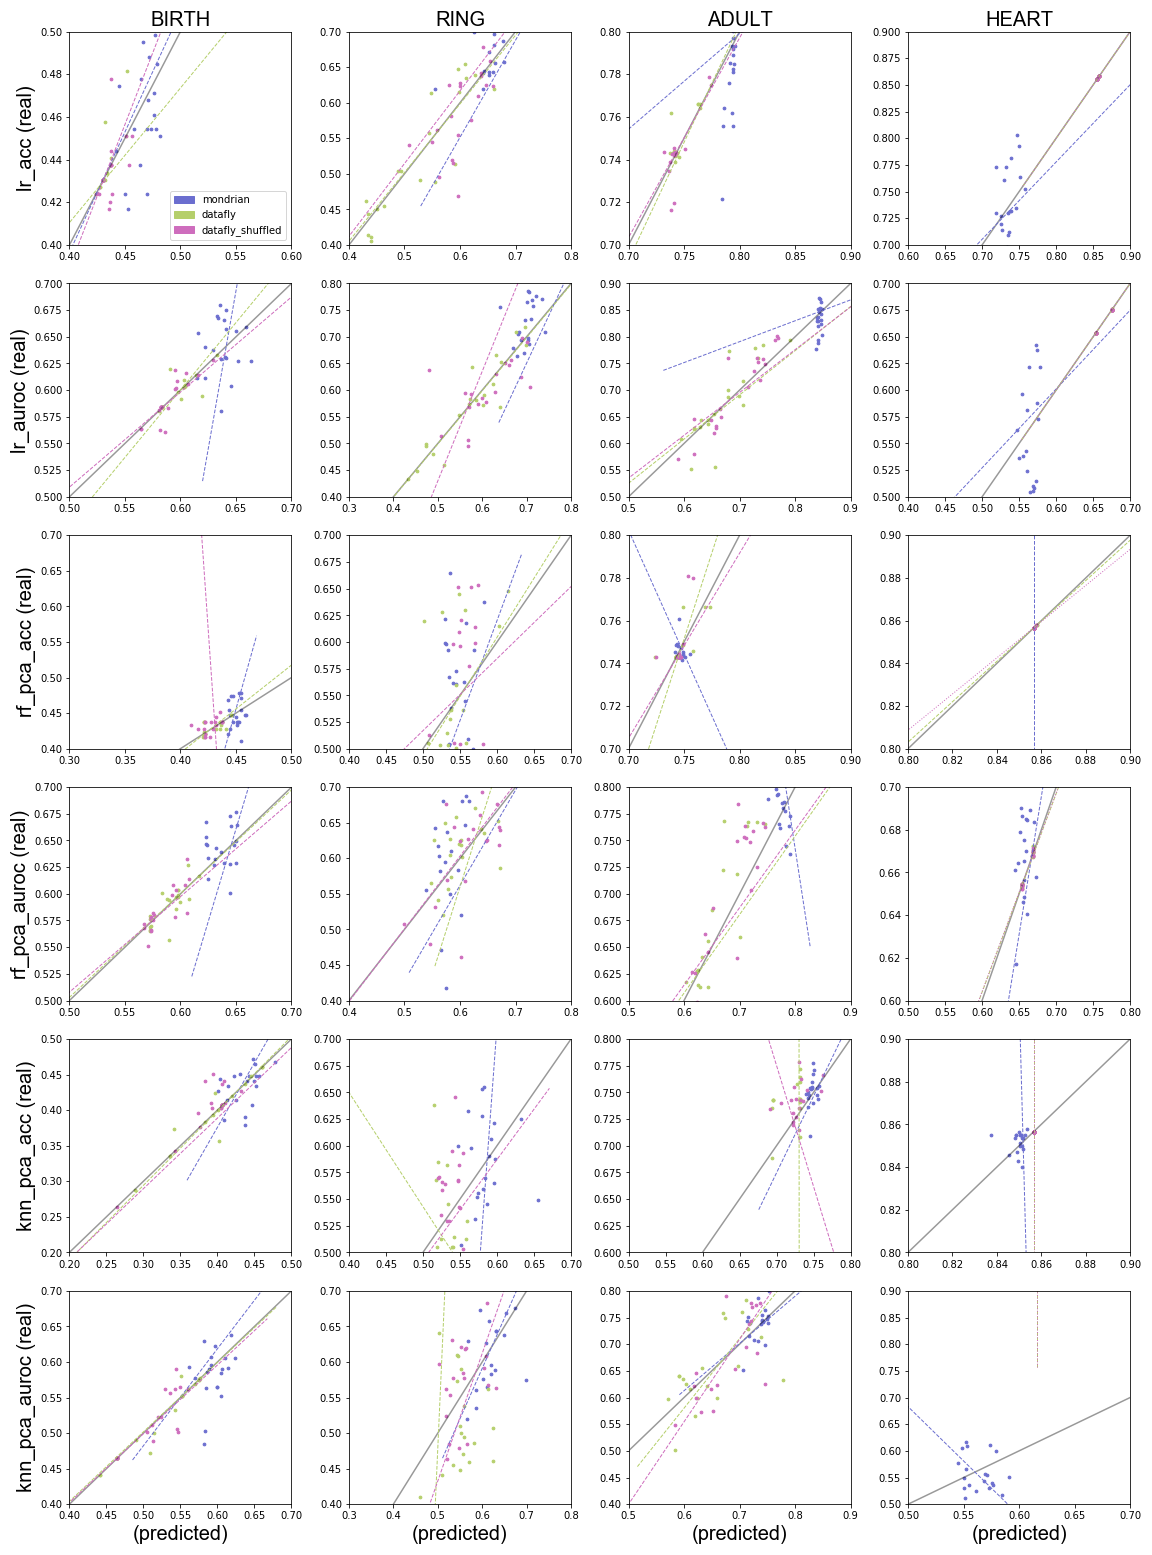
\includegraphics[width=\textwidth]{project/fig/megametrics-vs-accs_sep_trends.png}
    \caption{Scatterplots of the Meta-Metrics-- the trained Auto-Sklearn ensemble models-- predicting utility for the different algorithms on the different datasets. The different colors represent the different algorithms. The thin black line is the reference $y=x$ line, and the colored dashed lines are the trend lines for the scatters. The results show most Meta-Metrics predicting true utility reasonably accurately, with a few exceptions, notably on the heart datasets.}
    \label{fig:meta_scatter}
\end{figure}


\subsection{1v1 Meta-Metric Prediction}
As a more quantitative analysis of the Meta-Metrics, we replicate the method described in section \ref{sec:1v1_single}: when given two random datasets, what are the chances that the dataset with the highest Meta-Metric score is the one that is most ``useful''? We take the test set saved for every combination of algorithm, dataset, and utility measure, and compare the predicted utility to the measured utility. We then take the average of the results for the utility measures to aggregate by algorithm in Table \ref{tab:1v1_meta}. 

Depending on the dataset, we get different performances. We do not see much improvement on the ring dataset-- its highest single metric scored picked the most useful dataset 64.4\% percent of the time, and the combined metrics only increased that by 0.5\%. Adult has a lower average score than the single metric entropy for that dataset did. However, the average sees some improvement compared to its single metric results, averaging 66.7\% using the Meta-Metrics compared to a previous average of 60.5\%. Birth sees a larger increase, picking correct datasets about 76\% of times. The heart dataset once again scores better on all the algorithms than the others.

Putting things back into perspective, the Meta-Metrics generate an increase of the percent of times we pick the dataset with most measured utility, but still with mixed success. This is probably due to the noise we obtained, seen in the scatterplots. The overall trend is good, but when picking out a dataset from a handful of them, it becomes much harder. Considering that this is a best case scenario, the results paint a bleak picture for metrics.

\begin{table}[h]
\begin{tabular}{|l|c|}
\hline
\rowcolor{gray!50}
\cellcolor{gray!50} Dataset & Avg. Correctness  \\
\hline
\cellcolor{gray!50} birth   & 0.763 \\
\cellcolor{gray!50} ring    & 0.649 \\
\cellcolor{gray!50} adult   & 0.667 \\
\cellcolor{gray!50} heart   & 0.883 \\
\hline
\end{tabular}
\centering
\caption{A table displaying the rate of correctness of the 1v1 experiments on the Meta-Metrics. Here, we aggregate on the utility measures and algorithms to display results per dataset. Results show our Meta-Metrics predict more accurately than the individual metrics, but not by much.}
\label{tab:1v1_meta}
\end{table}




\subsection{Meta-Metric ``Transferability''}
Not only do we show that even the Meta-Metrics struggle to consistenly make good decisions, but we show that they become even more inconsistent as soon as we try to transfer their predictive powers to other tasks. To show the lack of Meta-Metric reusability, we tailor the 1v1 comparison method previously used. 

The intuition is as follows: if we cannot use a Meta-Metric trained to predict utility for Mondrian datasets to predict the best of two datasets that were anonymized using a Datafly algorithm (keeping the dataset type and utility measure constant), then the Meta-Metric is specific to Mondrian, and equally so for the other algorithms. This implies that if we wanted to use Meta-Metrics as utility metrics, we would need one Meta-Metric per algorithm in existence. 

On top of that, we need to ensure that the Meta-Metrics are also transferable to other dataset. In other words, using the Meta-Metric trained for a particular type of dataset (e.g., birth, ring,...), out of two datasets from another type of dataset, can we still apply our Meta-Metric to pick the most useful? If we cannot, that once again implies we need a Meta-Metric per type of existing dataset, of which there are infinitely many.

Finally, the same problem applies to the utility measure-- there are infinitely many classification tasks. If a Meta-Metric trained for a specific utility measure cannot be used to help predict other utility measures then the Meta-Metrics cannot be useful.

For Meta-Metrics to be useful as predictors of utility, we would need to show that they are transferable across three dimensions: algorithm used, dataset type, and utility measure. Therefore, we do three experiments:

\begin{itemize}
    \item Given two $k$-anonymous datasets anonymized using a specific algorithm, can we predict the one with more utility using a Meta-Metric trained on another algorithm?
    
    \item Given two $k$-anonymous datasets, can we predict the one with more utility using a Meta-Metric trained on another dataset?
    
    \item Given two $k$-anonymous datasets, can we predict which will have a better measured utility using a Meta-Metric trained for another utility measure?
\end{itemize}

We keep every dimension not being tested constant. For example, testing if the Meta-Metric trained on the Datafly algorithm transfers to the Mondrian and Datafly-Shuffled algorithm, we only test the Meta-Metric of the combination (Datafly $\times$ birth $\times$ lr\_acc) on $k$-anonymous versions of birth datasets, and using the lr\_acc utility measure.

All three questions result in the same answer: the Meta-Metrics cannot be transfered; taken out of their context, they do not have any use. 


\subsubsection{Are the Meta-Metrics transferable to other algorithms?}
To test if the Meta-Metrics trained on a specific algorithm are transferable, for every Meta-Metric trained on that algorithm, we filter the test metrics to those that were for different algorithms, but the same dataset. We then use the Meta-Metric to predict their utility, and ,for every pair of datasets, check to see if the one with the best predicted utility is the one that is truly most useful. Aggregating on all the datasets and utility measures, we find the percentage of time the Meta-Metrics correctly predict the most useful of two datasets. The information is displayed in Table \ref{tab:1v1_cross_algo}. 

The results show a lack of transferability for Mondrian Meta-Metrics to the other algorithms' datasets; they correctly identify the better dataset 60\% of the time (or about 10\% better than random). The Datafly algorithms are more transferable between each other which makes sense as they obtained similar results throughout our experiments. Nevertheless, because of the similarity of the results seen throughout this project, we would have expected the portability of the Datafly Meta-Metrics to and from the Datafly-Shuffled Meta-Metrics to be better. We conclude Meta-Metrics are algorithm specific.

\begin{table}[h]
\center
\begin{tabular}{|c|l|l|l|}
\hline
\rowcolor{gray!50}
Meta-Metric used \textbackslash used on  & mondrian & datafly & datafly\_shuffled \\
\hline
\cellcolor{gray!50} mondrian          & -        & 0.606   & 0.607             \\
\cellcolor{gray!50} datafly           & 0.668    & -       & 0.765             \\
\cellcolor{gray!50} datafly\_shuffled & 0.631    & 0.823   & -      \\
\hline
\end{tabular}
\caption{A table to show how often, when using the Meta-Metric for one algorithm, we could predict the most useful of two datasets that have been anonymized using another algorithm. We find that Mondrian does not predict Datafly datasets very well, and Datafly algorithms do not perform well on Mondrians either.}
\label{tab:1v1_cross_algo}
\end{table}

\subsubsection{Are the Meta-Metrics transferable to other datasets?}
We conduct a similar experiment for the transferability of Meta-Metrics to other datasets as we did for the transferability to other algorithms: we test how well the Meta-Metric for a dataset can predict the most useful of two datasets, of a different type, but anonymized by the same algorithm and with the same utility measure. We display the percentages obtain for the different Meta-Metrics in Table \ref{tab:1v1_cross_sets}.

The results show that the Meta-Metrics on one dataset struggle to make sense of the metrics calculated on another type of dataset, never scoring above 78.1\%. We come to the conclusion that Meta-Metrics are dataset specific as well.
\begin{table}[h]
    \center
    \begin{tabular}{|c|l|l|l|l|}
\hline
\rowcolor{gray!50}
Meta-Metric dataset \textbackslash used on & birth & ring  & adult & heart \\
\hline
\cellcolor{gray!50} birth   & -     & 0.567 & 0.583 & 0.719 \\
\cellcolor{gray!50} ring    & 0.696 & -     & 0.641 & 0.781 \\
\cellcolor{gray!50} adult   & 0.585 & 0.627 & -     & 0.75  \\
\cellcolor{gray!50} heart   & 0.723 & 0.671 & 0.75  & - \\
\hline
\end{tabular}
    \caption{A table to show how often, when using the Meta-Metric for one dataset, we could predict the most useful of two $k$-anonymous datasets from another original set. We find that the Meta-Metrics do not transfer well across dataset, as no score is above a 78\%.}
    \label{tab:1v1_cross_sets}
\end{table}

\subsubsection{Are the Meta-Metrics transferable to other utility measures?}
Finally, we test to see if training Meta-Metrics for one utility measure is enough or if they are task specific. We follow the same procedure as above, this time keeping the datasets and algorithms constant, and obtain the results displayed in Table \ref{tab:1v1_cross_measures}. These are condemning results for the usefulness of Meta-Metrics (and by implication information loss metrics in general): We see that no Meta-Metric trained for a certain type of utility measure can be used to pick a more useful dataset out of two for another measure. The best performing cross measure Meta-Metric barely scored 22\% better than random.

\begin{table}[h]
\centerfloat
\resizebox{\textwidth}{!}{%
\begin{tabular}{|c|l|l|l|l|l|l|}
\hline
\rowcolor{gray!50}
Meta-Metric used \textbackslash used to predict & lr\_acc & lr\_auroc & rf\_pca\_acc & rf\_pca\_auroc & knn\_pca\_acc & knn\_pca\_auroc \\ \hline
\cellcolor{gray!50} lr\_acc & - & 0.554 & 0.721 & 0.507 & 0.673  & 0.63 \\
\cellcolor{gray!50} lr\_auroc  & 0.611  & - & 0.696 & 0.696 & 0.642  & 0.58 \\
\cellcolor{gray!50} rf\_pca\_acc & 0.632  & 0.646  & - & 0.627 & 0.652  & 0.558 \\
\cellcolor{gray!50} rf\_pca\_auroc & 0.576   & 0.727 & 0.685 & - & 0.622  & 0.607  \\
\cellcolor{gray!50} knn\_pca\_acc & 0.705  & 0.648   & 0.708 & 0.623 & - & 0.638 \\
\cellcolor{gray!50} knn\_pca\_auroc & 0.643 & 0.701 & 0.723 & 0.701 & 0.645  & - \\ 
\hline
\end{tabular}}
\caption{A table to show how often, when using the Meta-Metric trained for one utility measure, we could predict the most useful of two $k$-anonymous datasets according to another utility measure. We find that the Meta-Metrics do not transfer well across dataset, as no score is above a 73\%.}
\label{tab:1v1_cross_measures}
\end{table}

These results imply that Meta-Metrics are not very versatile tools. They can only be used in the exact context they were trained for.



\subsection{Implications for Individual Information Loss Metrics}
The Auto-Sklearn models learned how to combine the strengths of every individual metric in an optimal way, and while on a specific task-- a combination of algorithm, dataset, and utility measure-- the resulting trends were promising, we show that, when used to pick a dataset from a handful of choices, their predictive power takes a hit.

As a result of our experiments, we show that we cannot use the Meta-Metrics created here on random $k$-anonymized datasets or for any other combination of algorithm, dataset, and classification task than those presented here. As such, we come to the conclusion that if even the Meta-Metrics cannot be used out of their context, then no single metric will be usable either as no single metric at its best is better than all the metrics at their best.
\chapter{Discussion}
This project constitutes an exploratory analysis into the broad topic of utility metrics. We propose preliminary evidence into the fact that they are not as predictive as many claim \cite{hellinger&biv, ambiguity_metric, cm_granularity_metric, distance_metrics, ilm,ambiguity_metric,dse_metric,entropy_measure} in what we believe to be an intuitive and practical experiment. We explain why we believe our arguments to be compelling, and address the limitations to our method, and results.


\section{Experiment Design}
\subsection{Datasets}
To avoid making our judgments on metrics based on a single dataset, we found four with very different characteristics. We believe these were enough to provide a more general idea of the how metrics behave. However, we found the heart dataset to perform very differently to the others. We weren't able to ascertain exactly that was the case but we think it might be due to its heavily unbalanced nature. A limitation of our method might, therefore, be that we should have picked datasets that had equivalent class distributions or to have balanced the classes before starting. 


\subsection{Anonymization}
We believe our method to be compelling as it addresses a lot of the components that form a $k$-anonymization: we look at the $k$ value, different algorithms, generalization trees (when relevant), and the datasets have varying sizes to account for the fact that $k$-anonymizations suppress relatively more information on smaller datasets than larger ones \cite{small_set_problem}. We further detail our thoughts on the different anonymization components:

\begin{itemize}
    \item \textbf{VGH Creation}: By creating random VGHs, not only does that allow for both good and bad generalization trees, leading to more range on the output metrics, but it removes the necessity for us to define a VGH ourselves, removing an external factor. Nevertheless, it's not without its drawbacks. Creating our random VGHs will lead to good and bad generalizations but it will lead to a lot of generalizations that would never be used in practice, which could reduce the applicability of our results. A possible, but probably infeasible, alternative would have been to collect all the available $k$-anonymous versions of the same datasets published by experts on the subject. This would have allowed us to study datasets that were totally relevant instead of ones that would never see the light of day anyway.
    \item \textbf{Choice of $k$}: We stand by the fact that $k$ was a more useful hyper-parameter when we varied it. However, the distribution used to choose the $k$ values was a bit arbitrary, and we still found some metrics that had very small ranges, particularly amongst the Mondrian.
    \item \textbf{Algorithms Used}: We picked two State-of-the-Art algorithms to test. We then added a variant of Datafly, Datafly-Shuffled, as a method to prove that if metrics couldn't distinguish between the utility of these then there was a problem. However, we ended up finding that the data destruction caused by Datafly algorithms was such that the two algorithms couldn't be differentiated. This rendered the Datafly-Shuffled datasets just as useful as the Datafly ones, which is to say not very. There are more powerful $k$-anonymity algorithms in literature but their implementations are not as widely spread \cite{ilm,samarati_algo, cm_granularity_metric}. Nevertheless, if we were to redo these experiments, we would pick an algorithm that uses VGHs more efficiently in the hopes to observe separate results for Datafly datasets and Datafly-Shuffled ones. This would be helpful because we could then justify that some metrics, like entropy, should not be able to distinguish between a sensible VGH, and an unordered one.
    \item \textbf{Additional Privacy Measure}: As mentioned in the background, $k$-anonymity by itself is not a sufficient privacy measure. As such, before applying the metrics, analysts would have to further anonymize the datasets, potentially affecting the results. For example, take the classification metric. It penalizes equivalence classes that have mixed labels in them. However, if we try to protect our dataset from Homogeneity attacks, we would drop equivalence classes that are-- in terms of classification-- 
   ``pure''. Thus, the better a $k$-anonymization manages to group records in way that make sense from a classification point of view, the more records will be dropped. Additionally, the resulting classification metric will be lower as all the pure equivalence classes will have been removed.
\end{itemize}

\subsection{Machine Learning Tasks}
We use a set of three different classifiers, and both AUROC and accuracies, to get some coverage of classification tasks in general. We avoid data pre-processing as much as possible but needed a PCA transformation for some of the classifiers to make the training times manageable. Although this gives us a good basis, we have to take into account that data can undergo pre-processing like balancing classes or selecting features, etc... . It's hard to say how that would affect the resulting utilities of the datasets.


Finally, in this project, we equate a dataset's utility to how well a classification task performs, trained on the dataset. This is a bit restrictive as there exist other uses for datasets that probably don't have the same requirements.

\subsection{Metrics Used}
We use a selection of metrics proposed in the literature. Particularly, we pick the ones that we find are often applied to be as relevant as possible. This is, of course, not an exhaustive list of metrics but it is definitely a good sample of them, and covers many different types.

\subsection{Meta-Metrics}
Until we added the Meta-Metrics, we only showed that individual metrics didn't have a linear correlation with utility. However, that never excluded some other relation from existing between the two, and that was a glaring limitation of this project. As an answer to that, we designed the Meta-Metrics experiment to ensure that even a trained ensemble model on all the metrics could not predict utility well. Because we can guarantee that an individual metric cannot perform better than the Meta-Metric (since it is a feature of the model), we can then show a maximum bound for the utility of an individual metric. Since even that is low, we can more safely say the link between metrics and utility is tenuous.

\subsection{1v1 Method Evaluation}
The 1v1 methods used to analyze results were an intuitive and quantitative way to assess the metrics' utility. Additionally, they emulated a realistic scenario that is at the core of how analysts use metrics. 
\chapter{Conclusion}

\section{Summary}
In this project, we proposed and carried out an analysis on the usefulness of information loss metrics as utility predictors. We first plot the utility of datasets against their corresponding metric results, and find little reason to believe the metrics to be good predictors for two reasons:

\begin{enumerate}
    \item we find that the trends are not consistent; they are different if we change the dataset used, the algorithm, or how we measure utility 
    \item For the metrics that were consistent, we found no linear correlation with the utility, making them useless predictors.
\end{enumerate}

The first is important because metrics are used as a benchmark to measure the quality of an anonymization (in terms of utility). Because we find no consistency over different tasks, one metric value might be very good for a task, but terrible for another, and we can't know that until we run a similar experiment to the one we did here for the dataset in question. In that case, metrics are not the time-saving measures for utility they were made out to be. For the few metrics that were consistent, the trends obtained gave little reason to believe in a linear correlation, implying that the utility measured was unrelated to the metrics, and vice versa.

We then derive a more quantitative measure of the metrics' usefulness in predicting utility by simulating a situation analysts will often find themselves in: we try to select the most useful dataset, out of two, basing ourselves on a metric. On most datasets, results show that using metrics granted marginally better selections, but, on average, by no more than 15\%.

The final component of the project involved the creation of Meta-Metrics, regressors in the form of ensemble models trained on the metrics obtained for our datasets. We use these Meta-Metrics to represent a best case scenario on how well the metrics can predict utility. Even in this case, we show limited transferability to other contexts, and limited predictive ability, with the Meta-Metrics adding less than 10\% accuracy to the average performances of individual metrics on the same datasets.



\section{Added Value}
Metrics are used as quality guarantees in anonymization processes everywhere, and so without question. Anonymization platforms, like ARX, use them \cite{arx}. So do researchers when trying to prove the data-preservation virtues of their new $k$-anonymization algorithms \cite{mondrian}.

Before this project, the only paper we found that compared a range of metrics just consisted in showing how the hyper-parameters of a $k$-anonymization impacted the metrics, taking for granted they were good predictors for utility \cite{systematic_comparisons_eval}. Instead, we take the opposite approach, measuring utility to test the metrics. Not only that, but we show that the foundations on which this was based is questionable. 

This project provides an exploratory analysis of whether metrics have the significance experts claim they do. Although our project is by no means perfect, it provides enough evidence to raise doubts on the usefulness of metrics, and warrant further research.


\section{Further Work}
As mentioned, this project opens the door for further research into the question. We could bolster the results provided during this project by looking into other State-of-the-Art algorithms. That would hopefully allow us to see difference between algorithms with shuffled VGHs and normal ones, and call out the metrics that can't distinguish between good and bad VGHs. We could also broaden the series of metrics tested, or confirm our results on more datasets. Lastly, we could add additional privacy measures to see how they affect utility, and if the metrics can predict that.

During the project, we raised a question on the effect an unbalanced $k$-anonymous dataset has on the utility of the metrics, and it remains unanswered for now. Finally, we can't help but wonder: considering the metrics we found were not good predictors for utility, could we develop one that is?


\appendix
\chapter{Additional Figures for Metric Trends on Different Algorithms}
\label{app:sep_trends_per_algo}
In this appendix, we add the Figures that we omitted in Section \ref{subsec:trends_datasets}, were we fit a line of best fir per algorithm per dataset in the scatterplots of the metrics for different utility measures. We see that per dataset, the trends are not always consistent, providing another argument as to why metrics do not have much value as general utility measuring tools.

\begin{figure}[!ht]
    \centering
    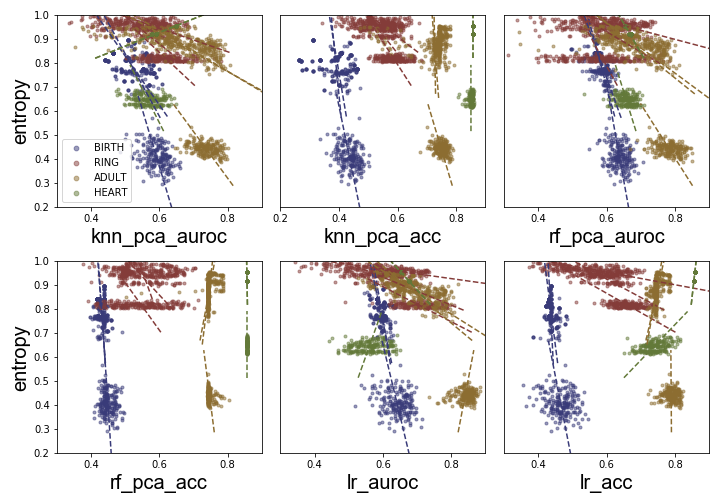
\includegraphics[width=0.8\textwidth]{project/fig/scatter_sep_trends/entropy_scatter.png}
    \caption{Scatterplots of the utility measures for the different classifiers against the entropy metric, separated by datasets. For every dataset, we draw a line of best fit per algorithm.}
\end{figure}

\begin{figure}[!ht]
    \centering
    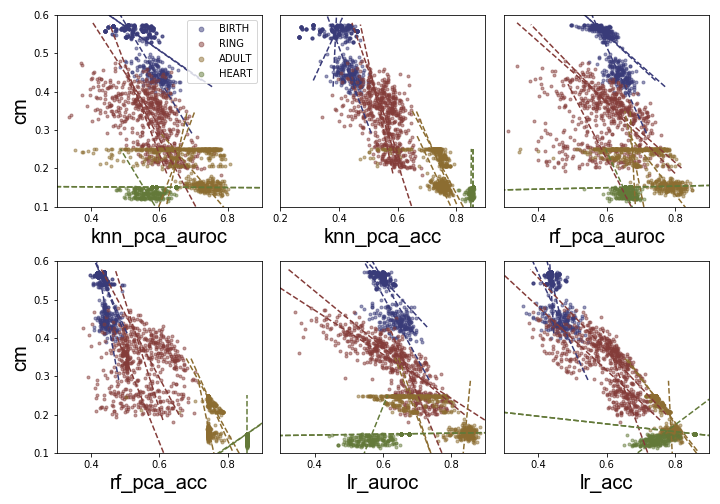
\includegraphics[width=0.8\textwidth]{project/fig/scatter_sep_trends/cm_scatter.png}
    \caption{Scatterplots of the utility measures for the different classifiers against the classification metric, separated by datasets. For every dataset, we draw a line of best fit per algorithm.}
\end{figure}

\begin{figure}[!ht]
    \centering
    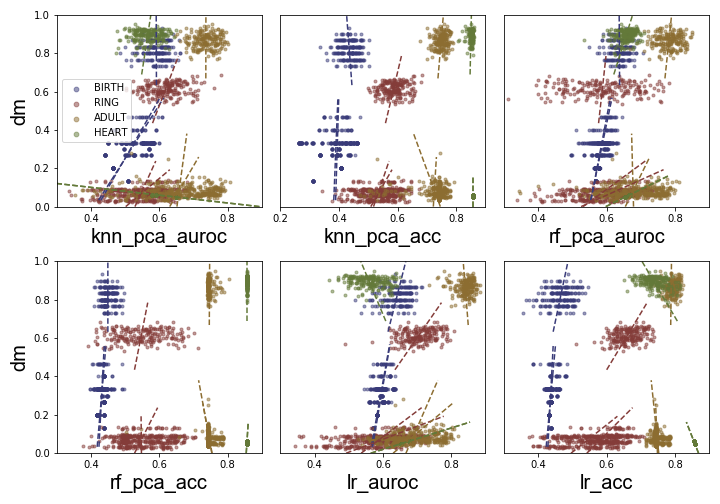
\includegraphics[width=0.8\textwidth]{project/fig/scatter_sep_trends/dm_scatter.png}
    \caption{Scatterplots of the utility measures for the different classifiers against the diameter metric, separated by datasets. For every dataset, we draw a line of best fit per algorithm.}
\end{figure}

\begin{figure}[!ht]
    \centering
    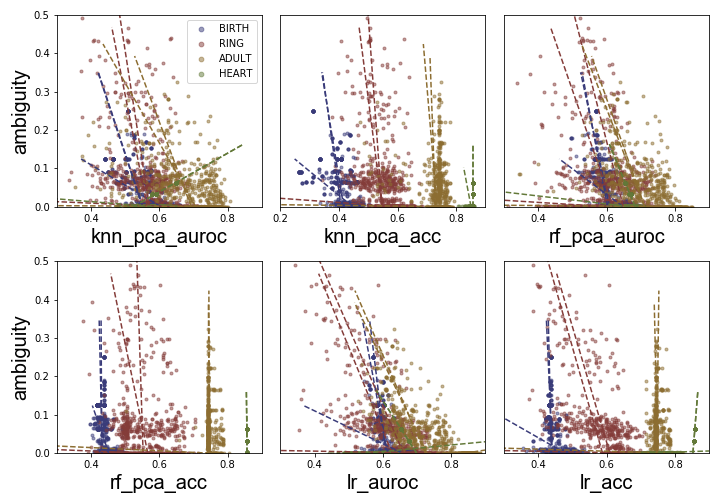
\includegraphics[width=0.8\textwidth]{project/fig/scatter_sep_trends/ambiguity_scatter.png}
    \caption{Scatterplots of the utility measures for the different classifiers against the ambiguity metric, separated by datasets. For every dataset, we draw a line of best fit per algorithm.}
\end{figure}

\begin{figure}[!ht]
    \centering
    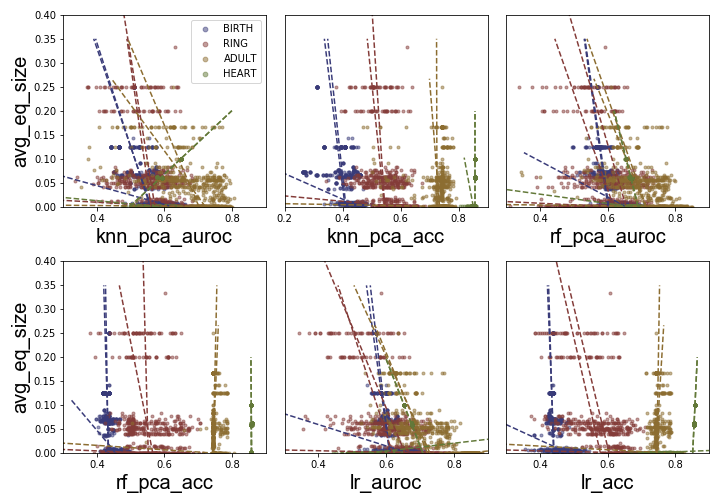
\includegraphics[width=0.8\textwidth]{project/fig/scatter_sep_trends/avg_eq_size_scatter.png}
    \caption{Scatterplots of the utility measures for the different classifiers against the average equivalence class size metric, separated by datasets. For every dataset, we draw a line of best fit per algorithm.}
\end{figure}

\begin{figure}[!ht]
    \centering
    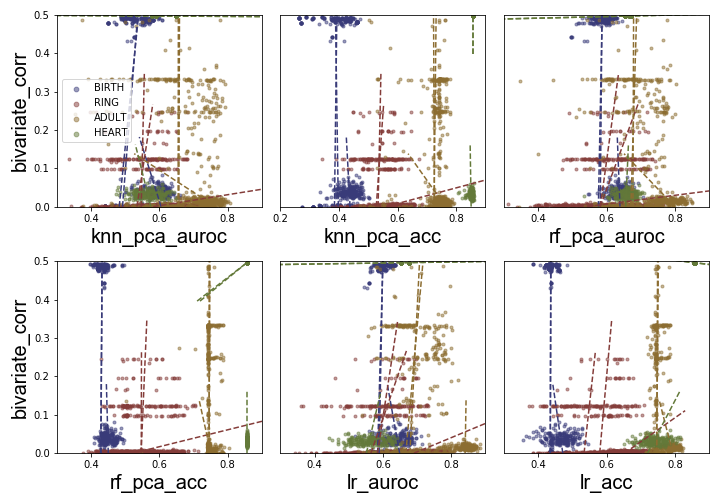
\includegraphics[width=0.8\textwidth]{project/fig/scatter_sep_trends/bivariate_corr_scatter.png}
    \caption{Scatterplots of the utility measures for the different classifiers against the bivariate correlation metric, separated by datasets. For every dataset, we draw a line of best fit per algorithm.}
\end{figure}

\begin{figure}[!ht]
    \centering
    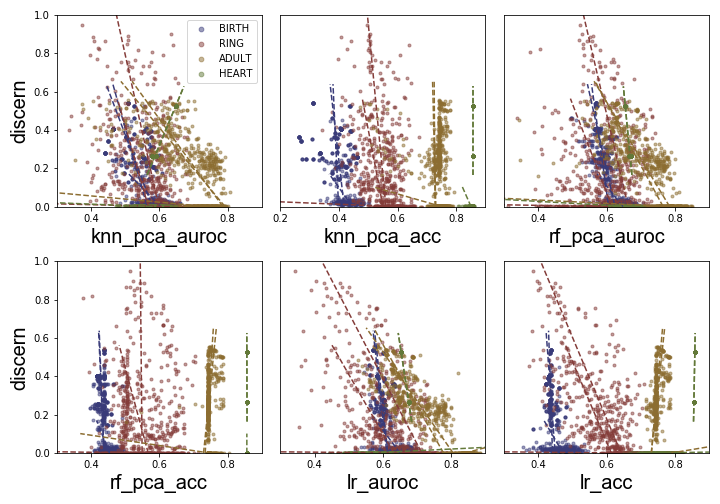
\includegraphics[width=0.8\textwidth]{project/fig/scatter_sep_trends/discern_scatter.png}
    \caption{Scatterplots of the utility measures for the different classifiers against the discernibility metric, separated by datasets. For every dataset, we draw a line of best fit per algorithm.}
\end{figure}

\begin{figure}[!ht]
    \centering
    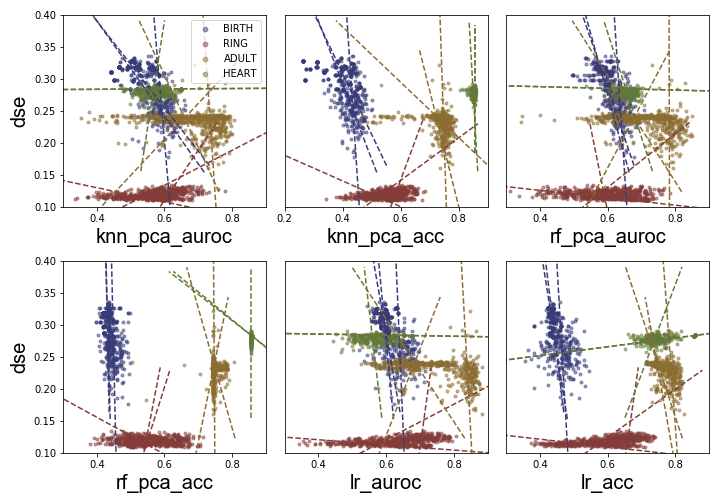
\includegraphics[width=0.8\textwidth]{project/fig/scatter_sep_trends/dse_scatter.png}
    \caption{Scatterplots of the utility measures for the different classifiers against the squared distance error metric, separated by datasets. For every dataset, we draw a line of best fit per algorithm.}
\end{figure}

\begin{figure}[!ht]
    \centering
    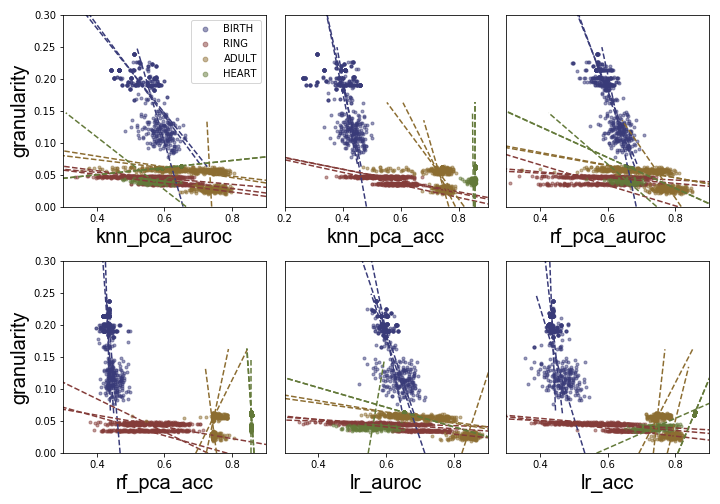
\includegraphics[width=0.8\textwidth]{project/fig/scatter_sep_trends/granularity_scatter.png}
    \caption{Scatterplots of the utility measures for the different classifiers against the granularity metric, separated by datasets. For every dataset, we draw a line of best fit per algorithm.}
\end{figure}

\begin{figure}[!ht]
    \centering
    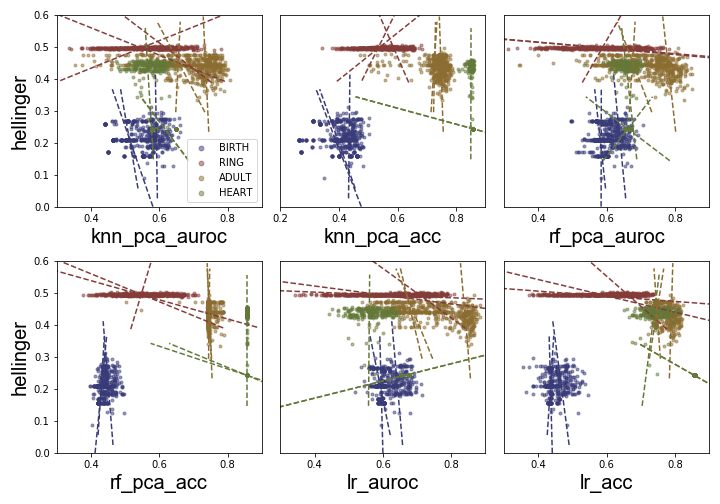
\includegraphics[width=0.8\textwidth]{project/fig/scatter_sep_trends/hellinger_scatter.png}
    \caption{Scatterplots of the utility measures for the different classifiers against the hellinger metric, separated by datasets. For every dataset, we draw a line of best fit per algorithm.}
\end{figure}

\begin{figure}[!ht]
    \centering
    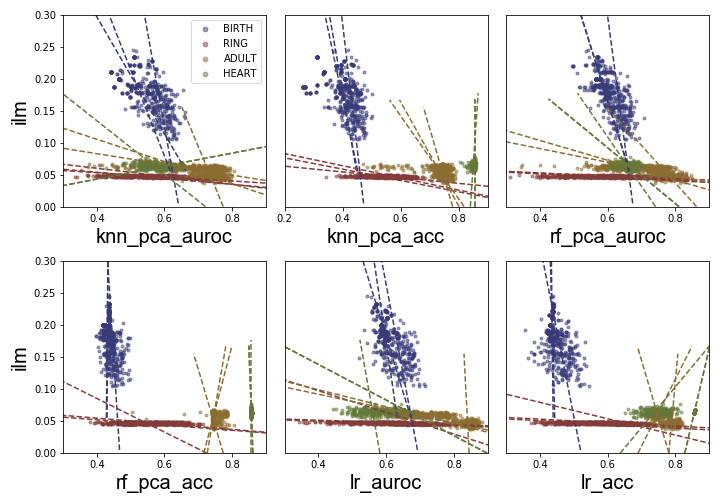
\includegraphics[width=0.8\textwidth]{project/fig/scatter_sep_trends/ilm_scatter.png}
    \caption{Scatterplots of the utility measures for the different classifiers against the information loss metric, separated by datasets. For every dataset, we draw a line of best fit per algorithm.}
\end{figure}

\bibliographystyle{unsrt}
\bibliography{bibs/sample}
\addcontentsline{toc}{chapter}{Bibliography}

\end{document}